\documentclass[12pt,letterpaper]{article}

\usepackage{amsmath, amsthm}
\usepackage{microtype, parskip}
\usepackage[comma,numbers,sort&compress]{natbib}
\usepackage{lineno}
\usepackage{docmute}
\usepackage{caption, subcaption, multirow, morefloats, rotating}
\usepackage{wrapfig}

\frenchspacing

\begin{document}

\section*{Results}

The results of the analyses described above take one of two forms: direct inspection of posterior parameter estimates, and downstream estimates of diversity and diversification rates based on posterior predictive simulations.

\subsection*{Posterior parameter estimates}

% look at the posterior predictive checks
%   which model has better fit
%   what does that mean?

The model used here in this study appears to have approximately adequate fit to the data based on the results of the posterior predictive check (Fig. \ref{fig:ppc}). Simulated datasets as estimated from the models' posterior appears similar in terms of average number of occurrences per species to the observed number of occurrences in the empirical mammal dataset.
\begin{figure}[ht]
  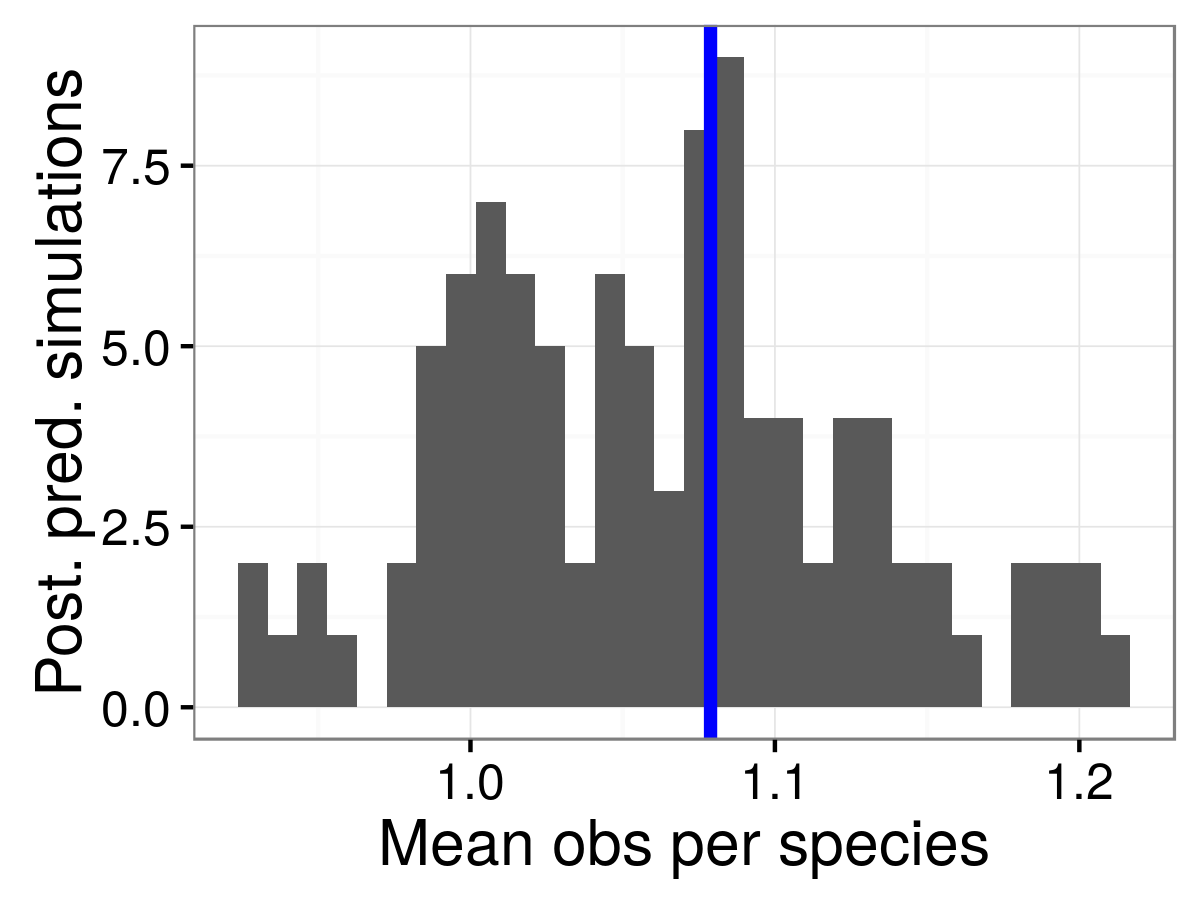
\includegraphics[width=\textwidth,height=0.3\textheight,keepaspectratio=true]{figure/pred_occ_bd}
  \caption[Posterior predictive check of average occurrence]{Comparison of the average observed number of occurrences per species (blue line) to the average number of occurrences from 100 posterior predictive datasets using the posterior estimates from the model used in this study. Adequate fit is indicated by the observed value of the test statistic being in the middle of the distribution of those calculated from the simulations.}
  \label{fig:ppc}
\end{figure}


% observation process
%   time
Log-odds of observing a species given that it is present varies greatly with time (Fig. \ref{fig:time_observe}) with lowest log-odds of observation being during the Gerigian and Harrisonian land-mammal ages. It is important to note, however, that all land-mammal ages with log-odds of observation greater than 2 have very high probabilities of observation, which means that while there may be large differences in log-odds of observation between land-mammal ages this may not translate to substantial difference in the probability of observation.
\begin{figure}[ht]
  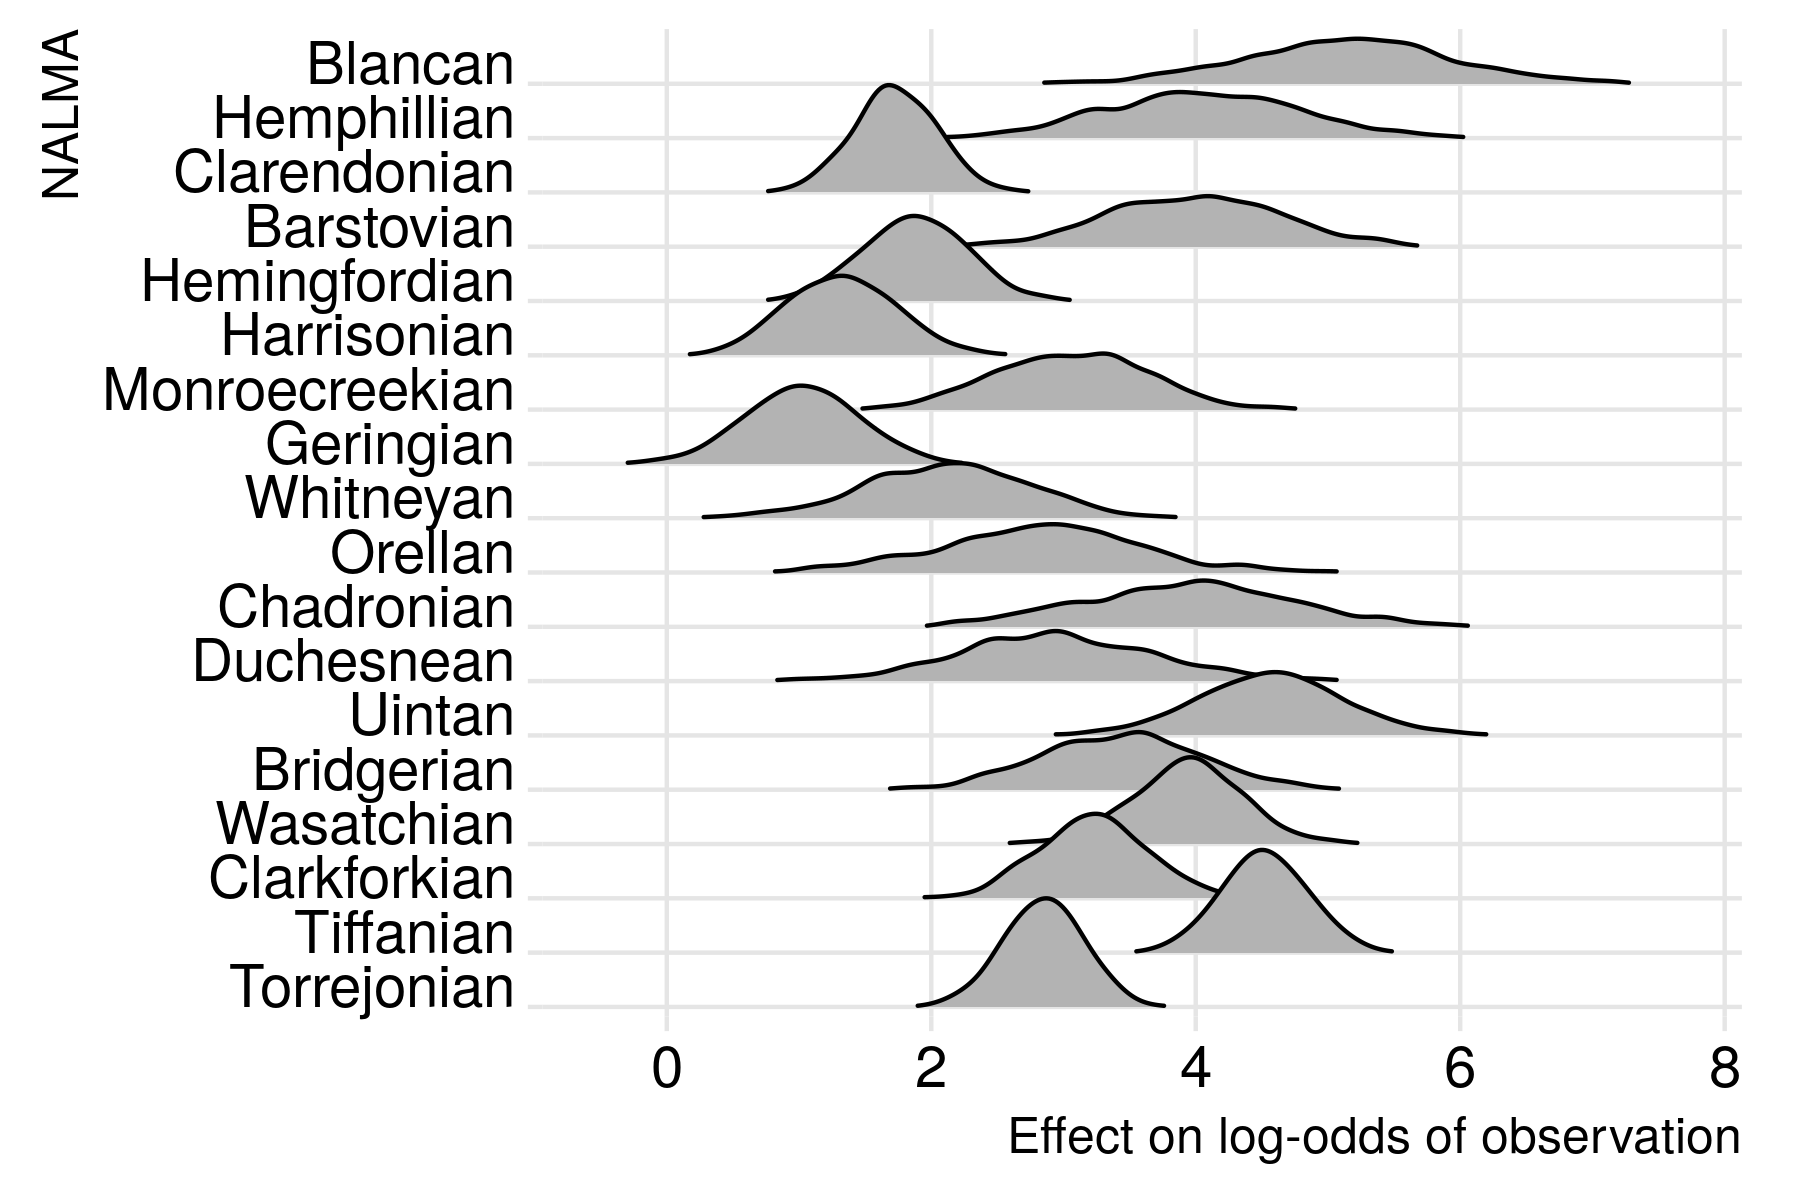
\includegraphics[width=\textwidth,height=0.4\textheight,keepaspectratio=true]{figure/time_observation}
  \caption{Ridgeline density plots of the estimates for the log-odds of observation from the time-varying intercept term. Each of the named time units are North American land-mammal ages. The oldest land-mammal age is at the bottom of the stack and the youngest is at the top.}
  \label{fig:time_observe}
\end{figure}

%   functional group
There is little variance in the effect of functional group on the log-odds of observing a species that is present (Fig. \ref{fig:fg_observe}). The only functional group with substantially less than expected log-odds of observation is scansorial insectivores, indicating that the fossil record of this group is the least complete of all the functional groups studied. Few functional groups have marginally better than expected log-odds of observation, the other insectivorous functional groups have marginally greater than average log-odds of observation; this is also the case for plantigrade omnivores. These results indicate that the observation histories of these functional groups are expected to be complete than most other functional groups. However, it is important to note that for many functional groups, their estimated log-odds of observation are poorly constrained with great uncertainty indicating little structure in how log-odds of observation varies between functional groups (Fig. \ref{fig:fg_observe}).
\begin{figure}[ht]
  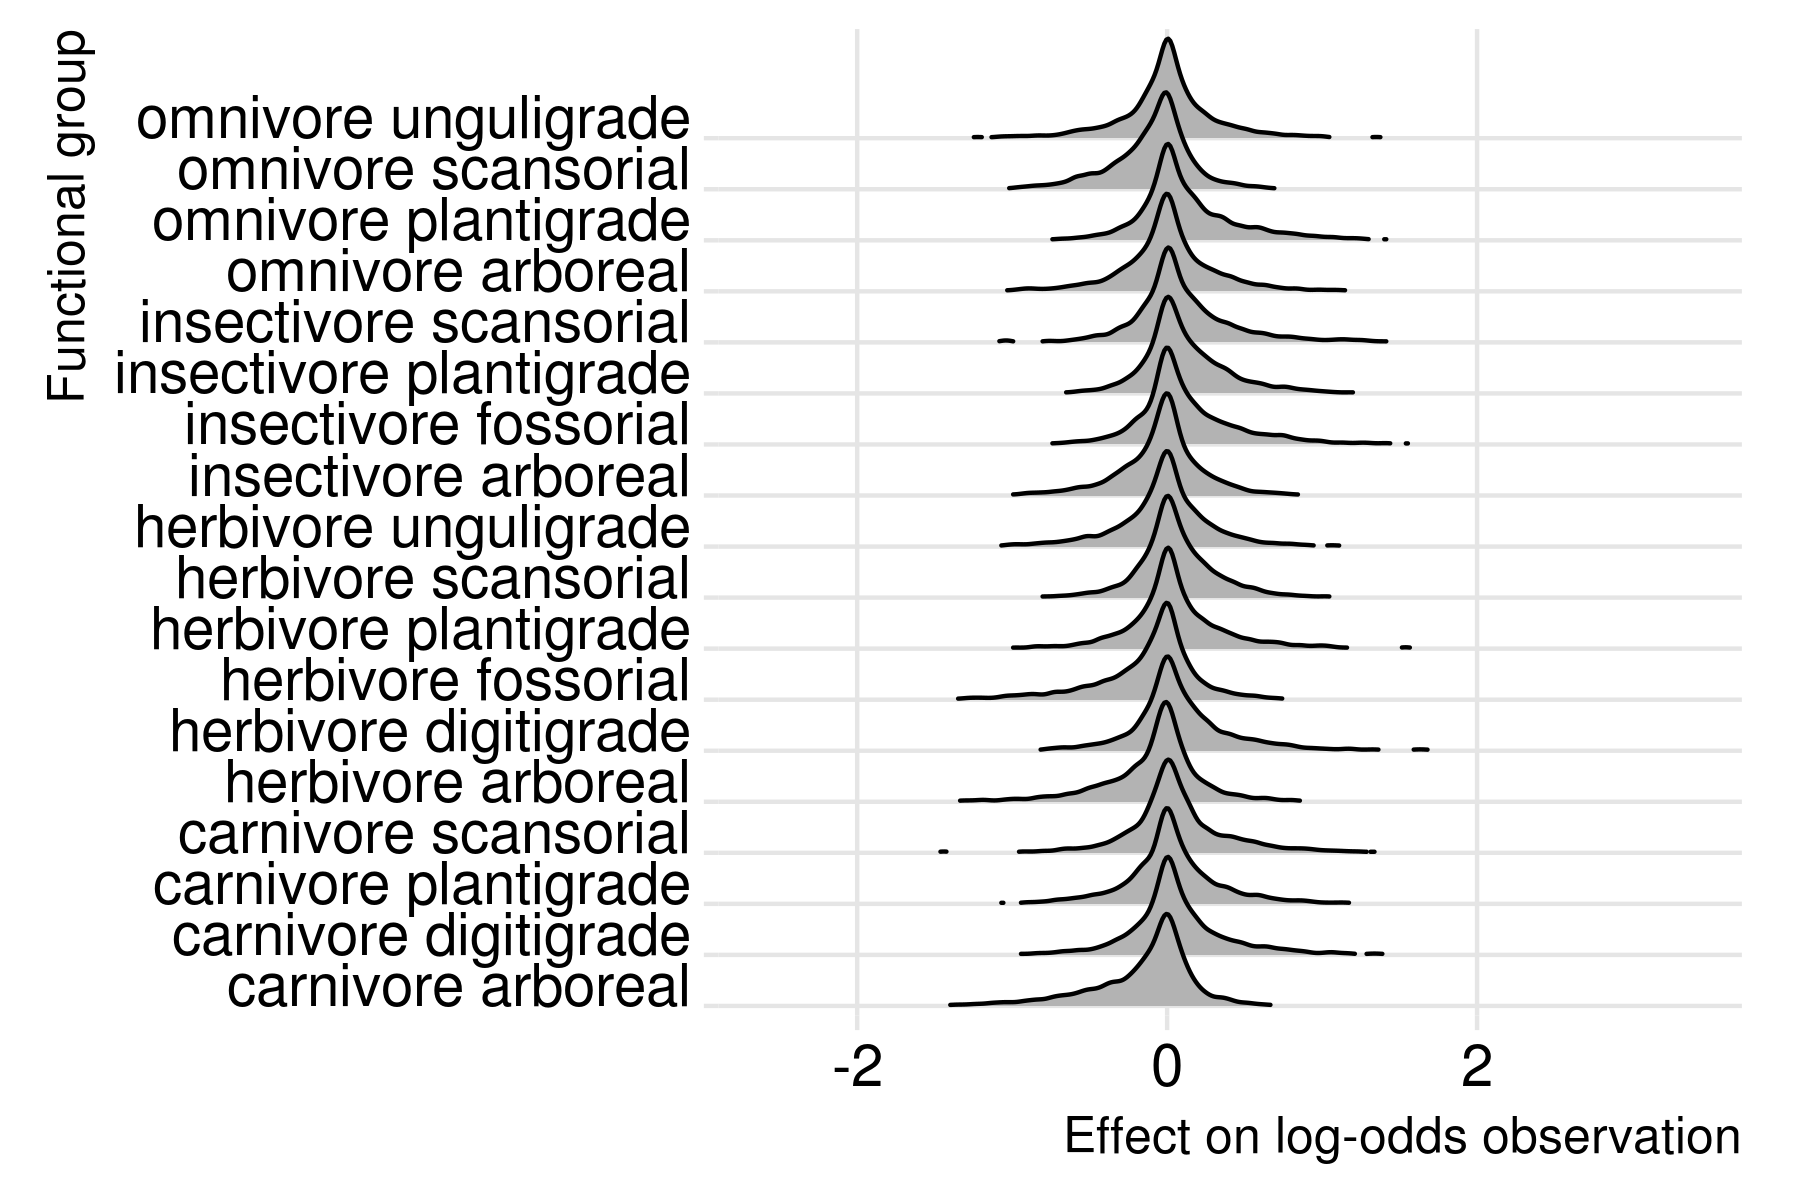
\includegraphics[width=\textwidth,height=0.4\textheight,keepaspectratio=true]{figure/ecotype_observation}
  \caption{Ridgeline density plots of the estimates of the effect of functional group on log-odds of observation. Each of the rows correspond to a different functional group as indicated by the dietary and locomotor category combination.}
  \label{fig:fg_observe}
\end{figure}

%   mass
Species mass is found to have a positive effect on probability of observing a species that is present (Fig. \ref{fig:mass_observe}). This result indicates that species with greater than average mass are expected to have more complete observation histories than species with less than average mass. However, this estimate does not translate to substantial differences in the estimated probability of observation because observation probability is so high for most of the Cenozoic (Fig. \ref{fig:time_observe}). In fact, it is only when land-mammal age observation probability is low that the effect of mass is observable. It is important to remember the effect of mass on observation was considered constant over time and that all differences observation probability between land-mammal ages is driven by variation over time. When log-odds of observation is high, differences due to covariate effects translate to very small differences in actual probability. % change this to just a single response curve? i like that i can visualize how little mass matters depending on overall prob of observation
\begin{figure}[ht]
  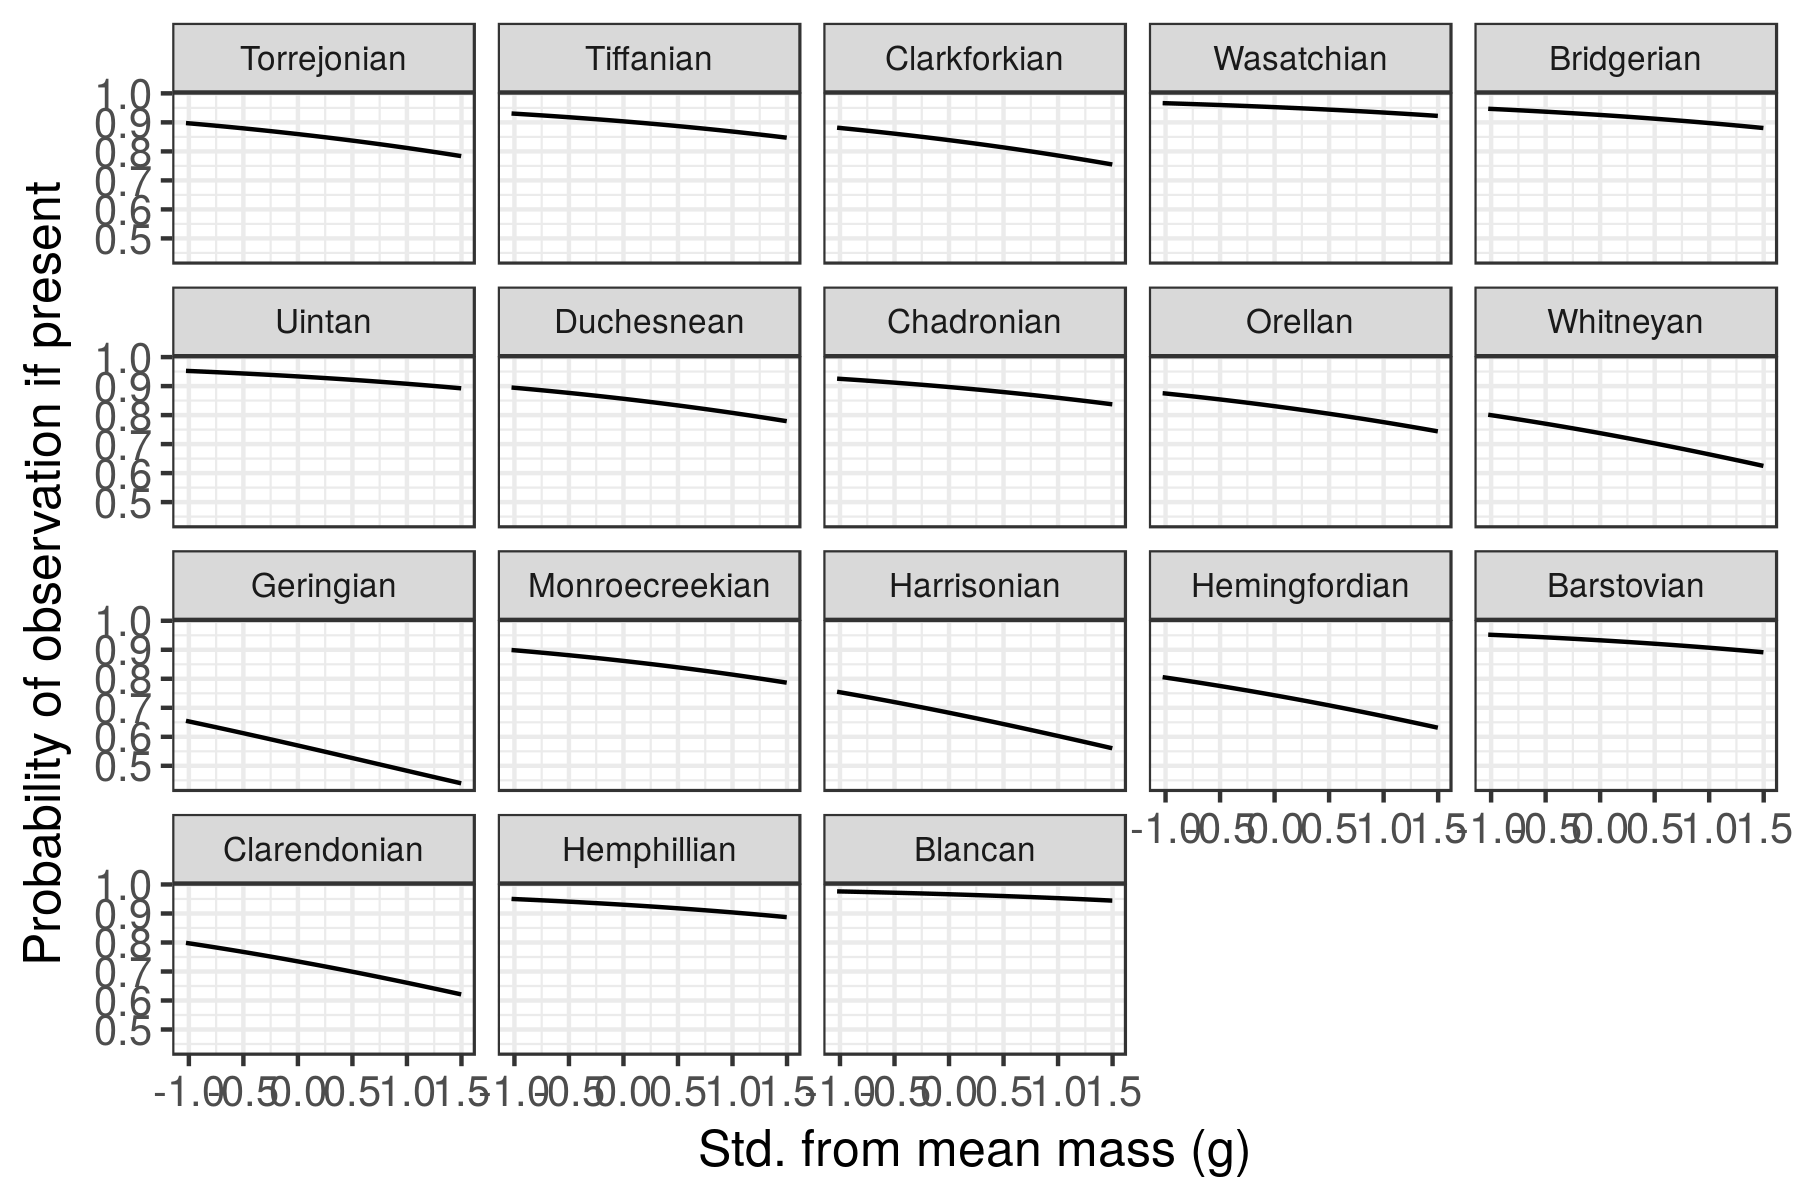
\includegraphics[width=\textwidth,height=0.4\textheight,keepaspectratio=true]{figure/mass_on_pres_bd}
  \caption[Estimates of the effect of mass on observation probability]{Estimates of the effect of species mass on probability of sampling a present species (\(p\)). Mass has been log-transformed, centered, and rescaled; this means that a mass of 0 corresponds to the mean of log-mass of all observed species and that mass is in standard deviation units. Probability of observation is presented for each of the NALMAs where the differences in mean probability of observation are due to variation between the time units (Fig. \ref{fig:time_observe}).}
  \label{fig:mass_observe}
\end{figure}


% origination
%   individual-level
%     FG time series
Origination probability varies greatly among functional groups with each functional group exhibiting a unique time series with a few shared features (Fig. \ref{fig:eco_origin}). When origination probability is below 0.50 this means that few if any new species of that functional group are entering the species pool, and when origination probability is greater than 0.50 new species of that functional group are probably entering the species pool. Finally, if origination probability is approximately 0.50, this indicates that it is equally likely that a new species is entering the species pool as that it is not. The slope of origination probability time-series is also very revealing; when the slope of the time series is positive then new species are being continually being added to the species pool, and when the slope is negative then the number of new species entering the pool is decreasing with time.

Most of the functional groups have peak origination probability at the present (Fig. \ref{fig:eco_origin}); new species in these functional groups are continually being added to the species pool. In the case of some functional groups,  such as digitigrade carnivores and fossorial herbivores, this is the culmination of those groups continued growth in the species pool. For other functional groups, such as arboreal herbivores, this peak is a reversal from previously relatively low origination probability; this indicates an expansion of these functional groups following a retraction.

Five of the functional groups have peak origination probabilities not at the present: arboreal carnivores, arboreal insectivores, plantigrade insectivores, scansorial insectivores, and unguligrade omnivores. The arboreal functional groups reach peak origination probability in the Paleogene, after which their origination probabilities approach and remain at 0.50, reflecting the loss of these functional groups from the species pool as origination probability never again increases. Additionally, the uncertainty surrounding in the estimates of origination probability is very large, especially in the Neogene. Large uncertainty in probabilities can reflect complete separation which results from that functional group leaving the species pool and it's (lack of) occurrence is without ambiguity CITATION. The patterns evinced by the other functional groups have similar properties but reach peak origination probability early in the Neogene. Interestingly, origination probability of scansorial insectivores has effectively two peaks, once in the late Paleogene and again in the early Neogene. Additionally, as will be discussed later in the context of standing diversity, all five of these functional groups decrease in diversity through the Cenozoic. 
\begin{figure}[ht]
  \centering
  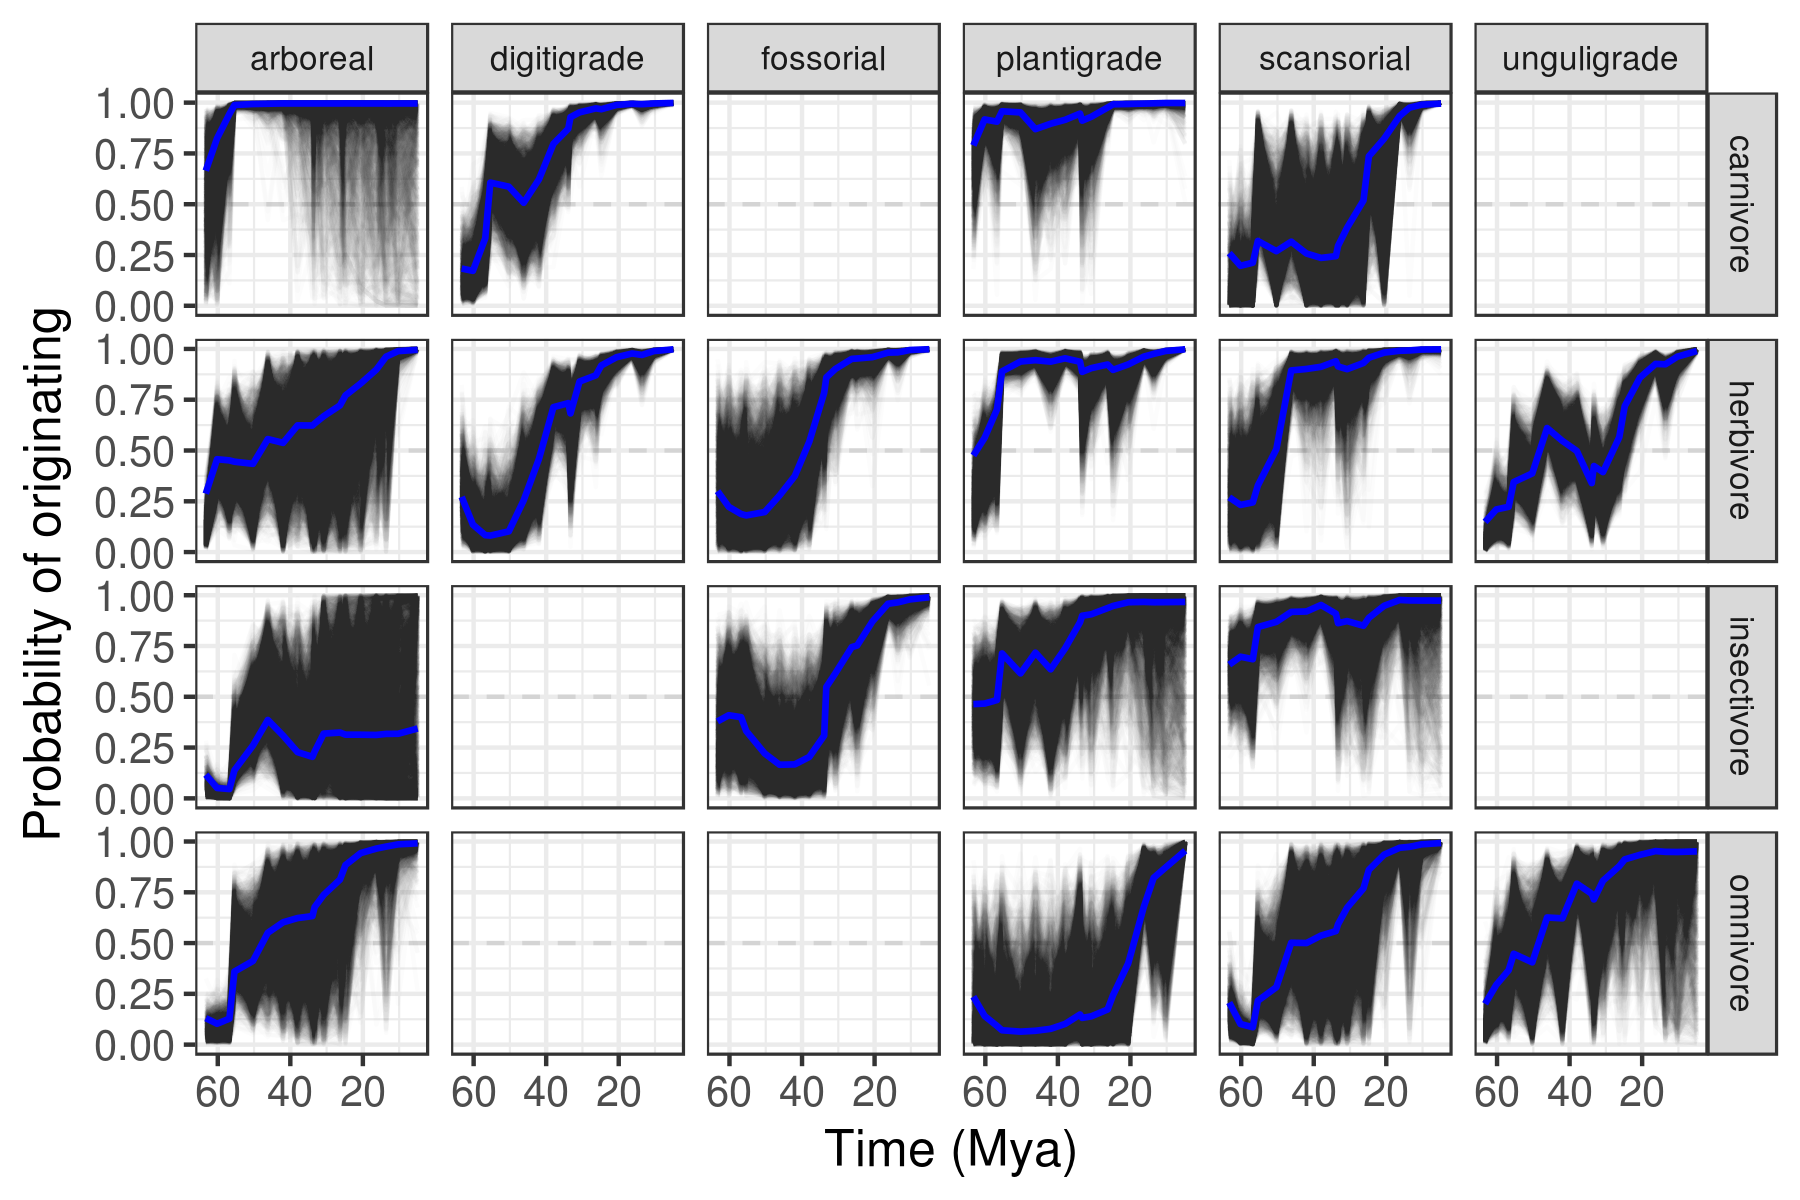
\includegraphics[width=\textwidth,height=0.4\textheight,keepaspectratio=true]{figure/ecotype_origin_bd}
  \caption[Estimates of functional group origination probability]{Probability of a mammal functional origination at each time point. Each panel depicts 100 time-series sampled from the model's posterior. The blue line is the mean origination probability as predicted by the group-level predictors. The columns are by locomotor category and rows by dietary category; their intersections are the observed and analyzed ecotypes. }
  \label{fig:eco_origin}
\end{figure}

%     order effect
Origination probability varies greatly amongst mammal orders (Fig. \ref{fig:order_origin}). These estimates reflect differences origination probability as well as the relative rarity of that order in the fossil record; if members of that order appear infrequently, they must have lower probability of origination. Orders with greater than average log-odds of origination include Multituberculata, Dinocerata, Didelphimorphia, Creodonta, Condylarthra, Cimolesta, and Acreodi. These orders are major components of the Paleogene fossil record. Orders with lower than average log-odds of origination include Rodentia, Pilosa, Lagomorpha, Eulipotyphyla, Cingulata, Carnivora, and Artiodactyla. These orders are characterized by small body size or primarily Neogene records. Additionally, the variance between orders is vary large ranging from -3 to 3 log-odds of origination; this large of variance reflects how species within these orders have very different patterns of origination independent from their origination based on functional ecology (Fig. \ref{fig:eco_origin}).
\begin{figure}[ht]
  \centering
  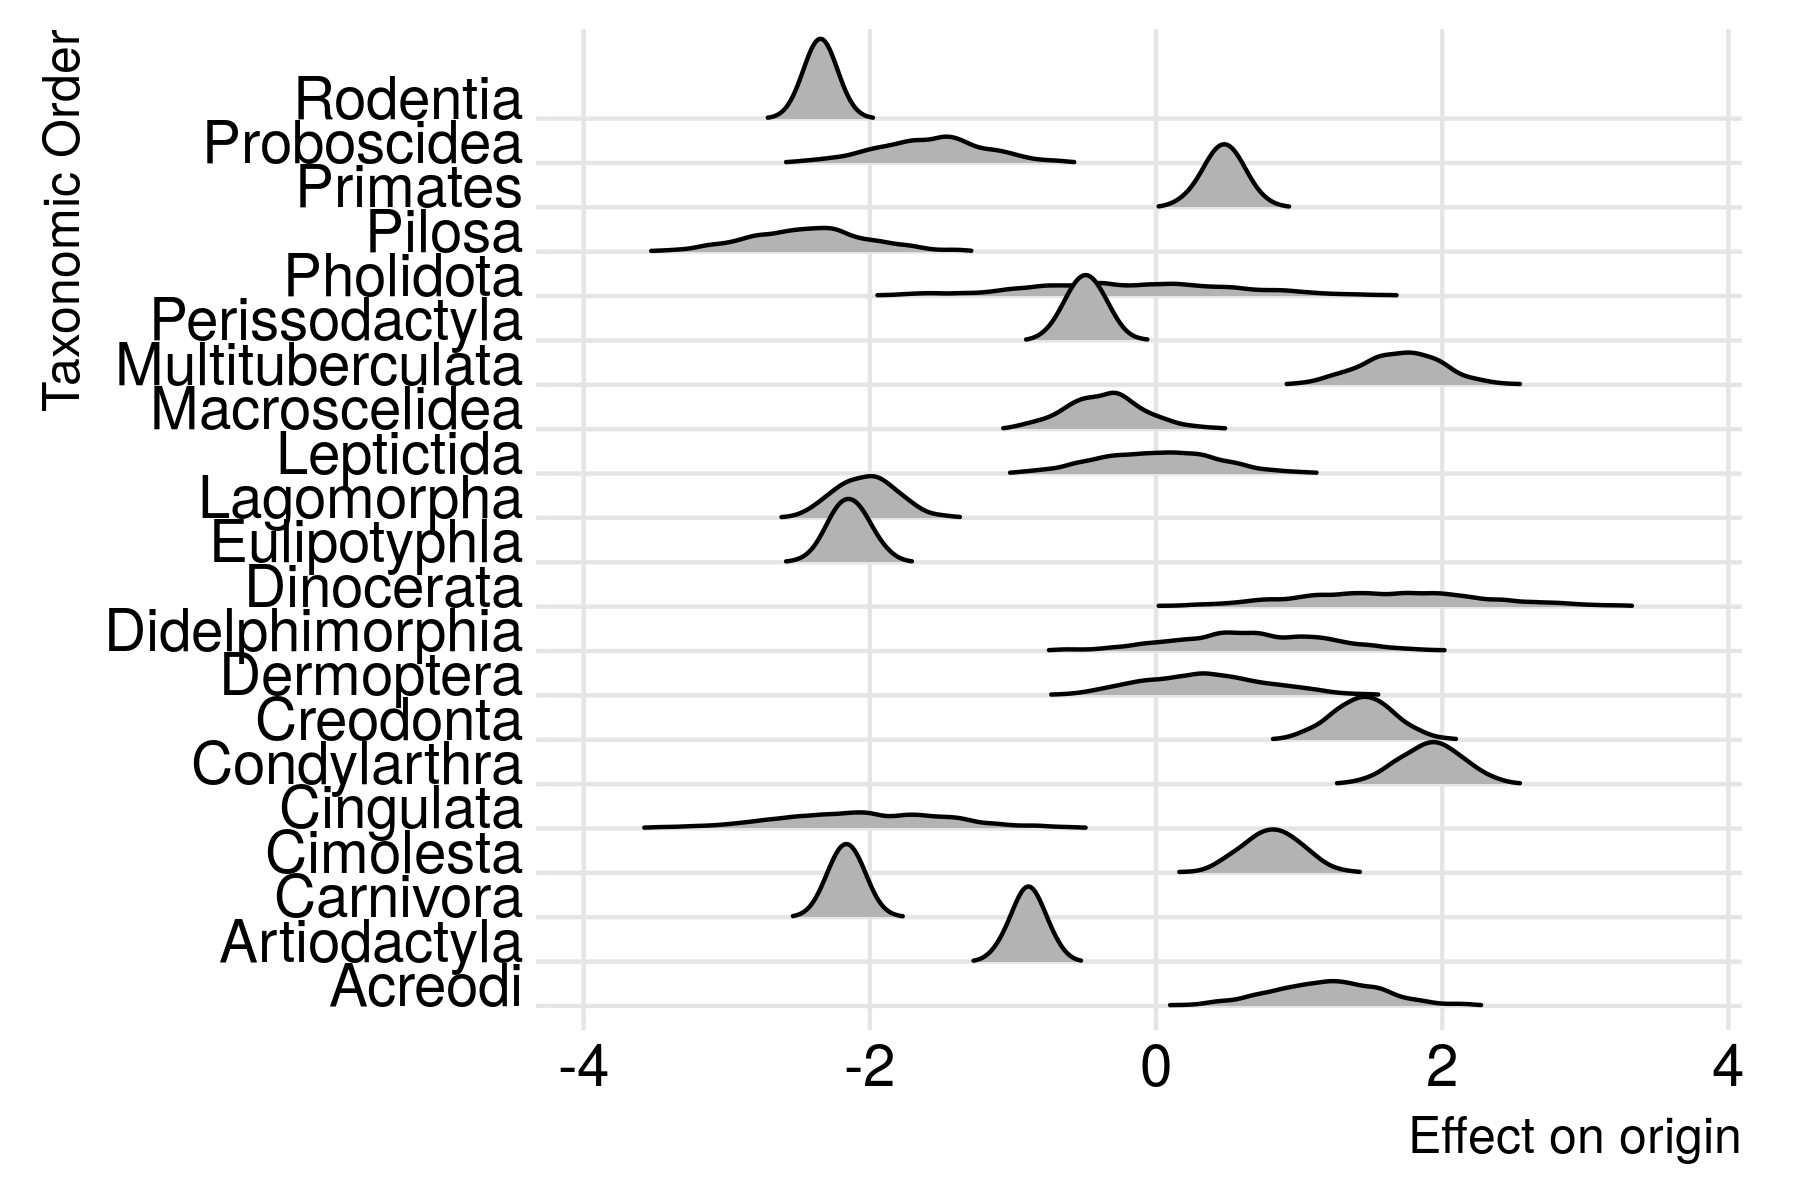
\includegraphics[width=\textwidth,height=0.4\textheight,keepaspectratio=true]{figure/order_origin_bd}
  \caption{Differences in log-odds of origination based on mammal orders. Positive values correspond to greater log-odds origination than average, while negative values correspond to lower log-odds of origination than average. These estimates reflect the rarity of that order in the fossil record as well as differences in origination.}
  \label{fig:order_origin}
\end{figure}

%     mass effect
Species mass is estimated to have a negative relationship with origination probability (Fig. \ref{fig:mass_origin}). This result means that species with greater than average mass have a lower probability of originating than species with a below average mass. This result is sensible given the left-skewed distribution of mammal species body sizes where large body sizes form the right-hand tail. There are fewer large body-sized mammals which have originated than small body sized mammals. Interestingly, many of the orders with small body sizes (e.g. Rodentia, Lagomorpha) have below average probabilities of originating (Fig. \ref{fig:order_origin}); while not completely kosher, when this result is considered together with the effect of mass on origination these effects could be counteracting each other. These results continue to add to the understanding of the heterogeneity and nuance associated with species origination dynamics.
\begin{figure}[ht]
  \centering
  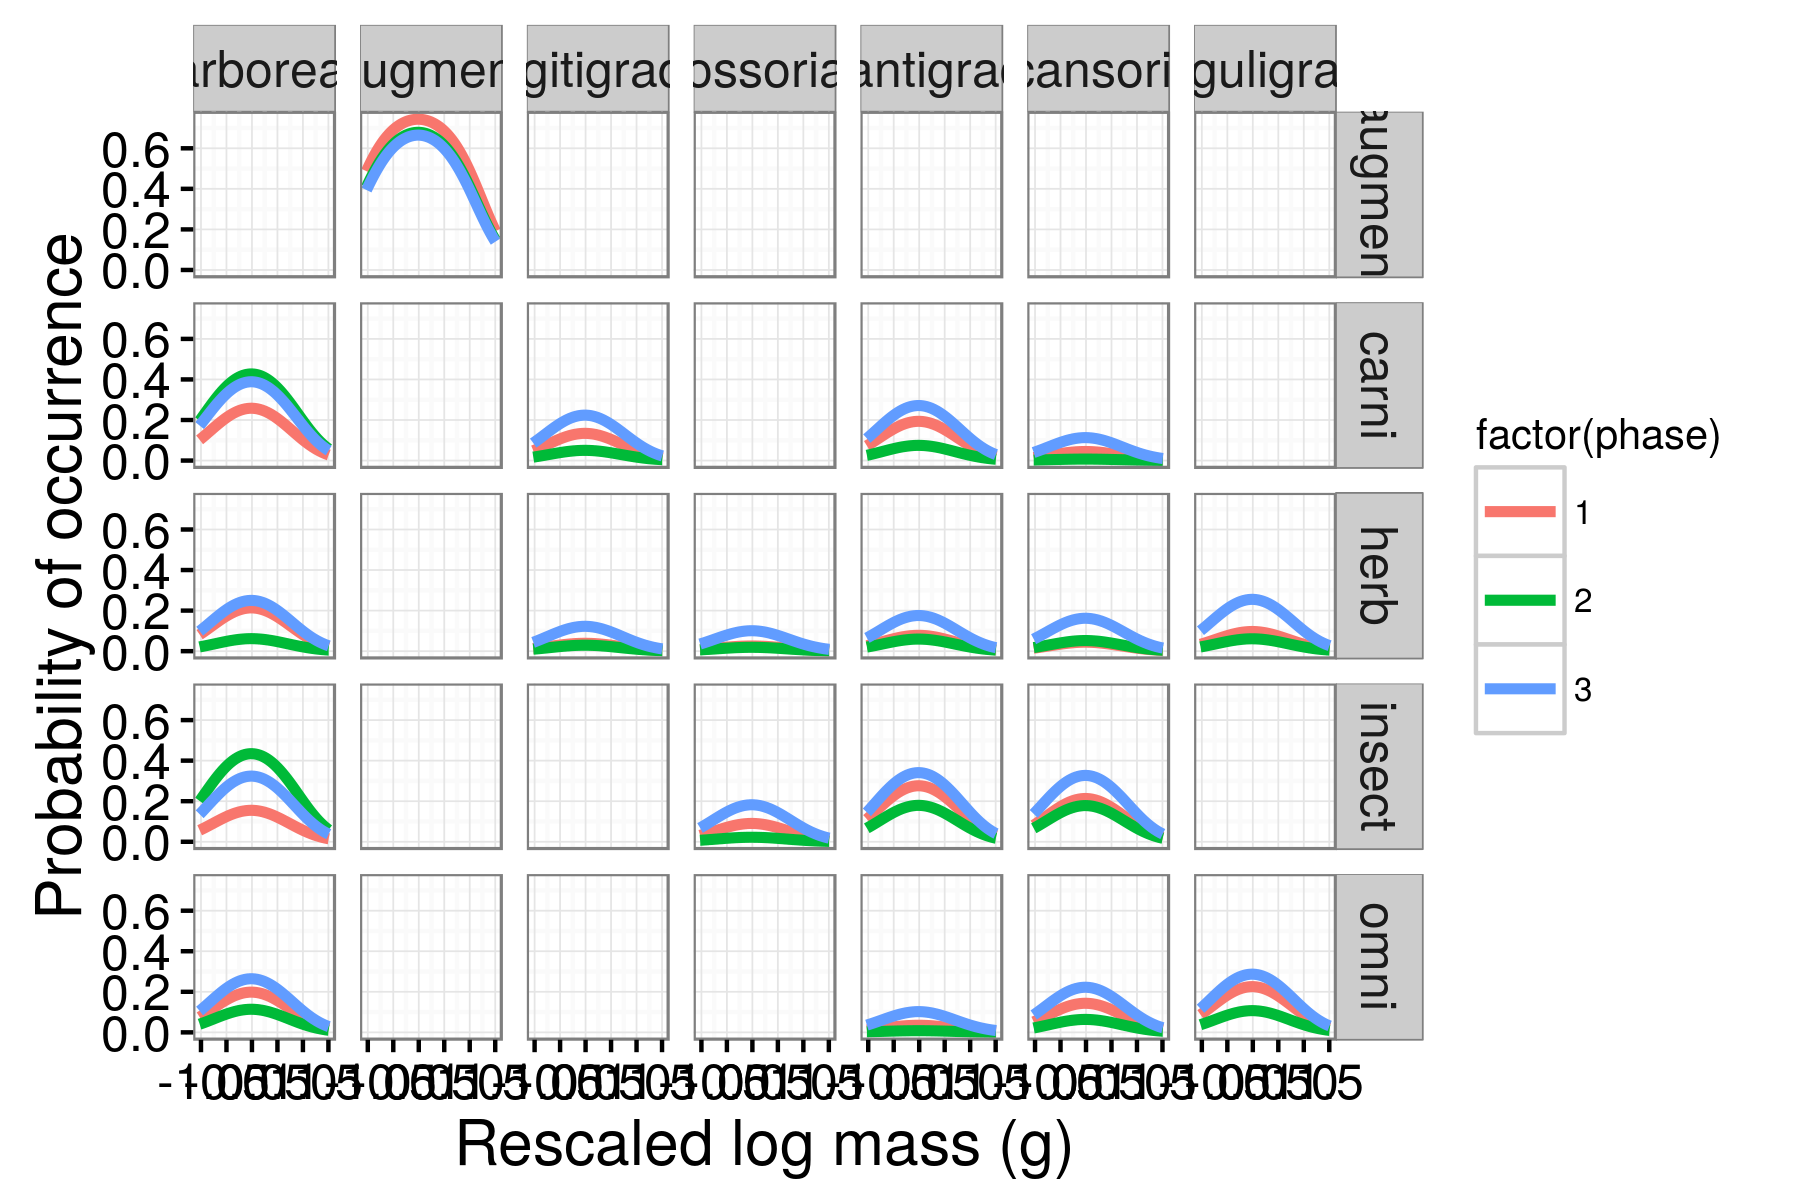
\includegraphics[width=\textwidth,height=0.4\textheight,keepaspectratio=true]{figure/mass_on_origin_bd}
  \caption[Effect of mass on probability of species origination as estimated from the birth-death model]{Mean estimate of the effect of species mass on the probability of a species originating for each of the three plant phases. The effect of mass is considered constant over time and that the only aspect of the model that changes with plant phase is the intercept of the relationship between mass and origination. The three plant phases are indicated by the color of the line. Mass has been log-transformed, centered, and rescaled; this means that a mass of 0 corresponds to the mean of log-mass of all observed species and that mass is in standard deviation units. For clarity, only the mean estimates of the effects of mass and plant phase are plotted.}
  \label{fig:mass_origin}
\end{figure}

%   group-level
%     temperature and plant phase
The group-level covariates are estimated with high probability (\(>\) 0.80) of being different from 0 (Fig. \ref{fig:group_origin_bd}). These results mean that the environmental factors analyzed here are expected to shape changes in origination probability over time. Importantly, the plant phases and global temperature are estimated to affect many of the functional groups

At least two of the three plant phases are associated with differences in origination probability for 14 of the 18 functional groups (\(> 0.85\) probability; Table \ref{tab:origin_plant}). The Paleocene-Eocene phase is found to be associated with differences in origination probability from the Miocene-Pleistocene for ten of the functional groups, all of which are expected to have lower origination probability than the latter (Table \ref{tab:origin_plant}). The Eocene-Miocene phase is found to be associated with differences in origination probability from the Miocene-Pleistocene for nine of functional groups: eight with a greater origination probability than the latter, and one with a lower origination probability than the latter (Table \ref{tab:origin_plant}). The Eocene-Miocene phase is expected to be assocaited with a greater origination probability than the Paleocene-Eocene for 13 of the functional groups (Table \ref{tab:origin_plant}). 

Temperature is estimated with \(> 0.85)\) probability to have an affect origination probability for ten of the 18 functional groups (Table \ref{tab:origin_temp}). In all cases this relationship is estimated to be negative, meaning that an increase in temperature is associated with a decrease in origination probability. Considering that, on average, temperature decreases through the Cenozoic CITATION, this implies that the origination probability of these ten functional groups may be tracking this long-term trend as opposed to the other functional groups which increases in origination probability independently of temperature.
\begin{figure}[ht]
  \centering
  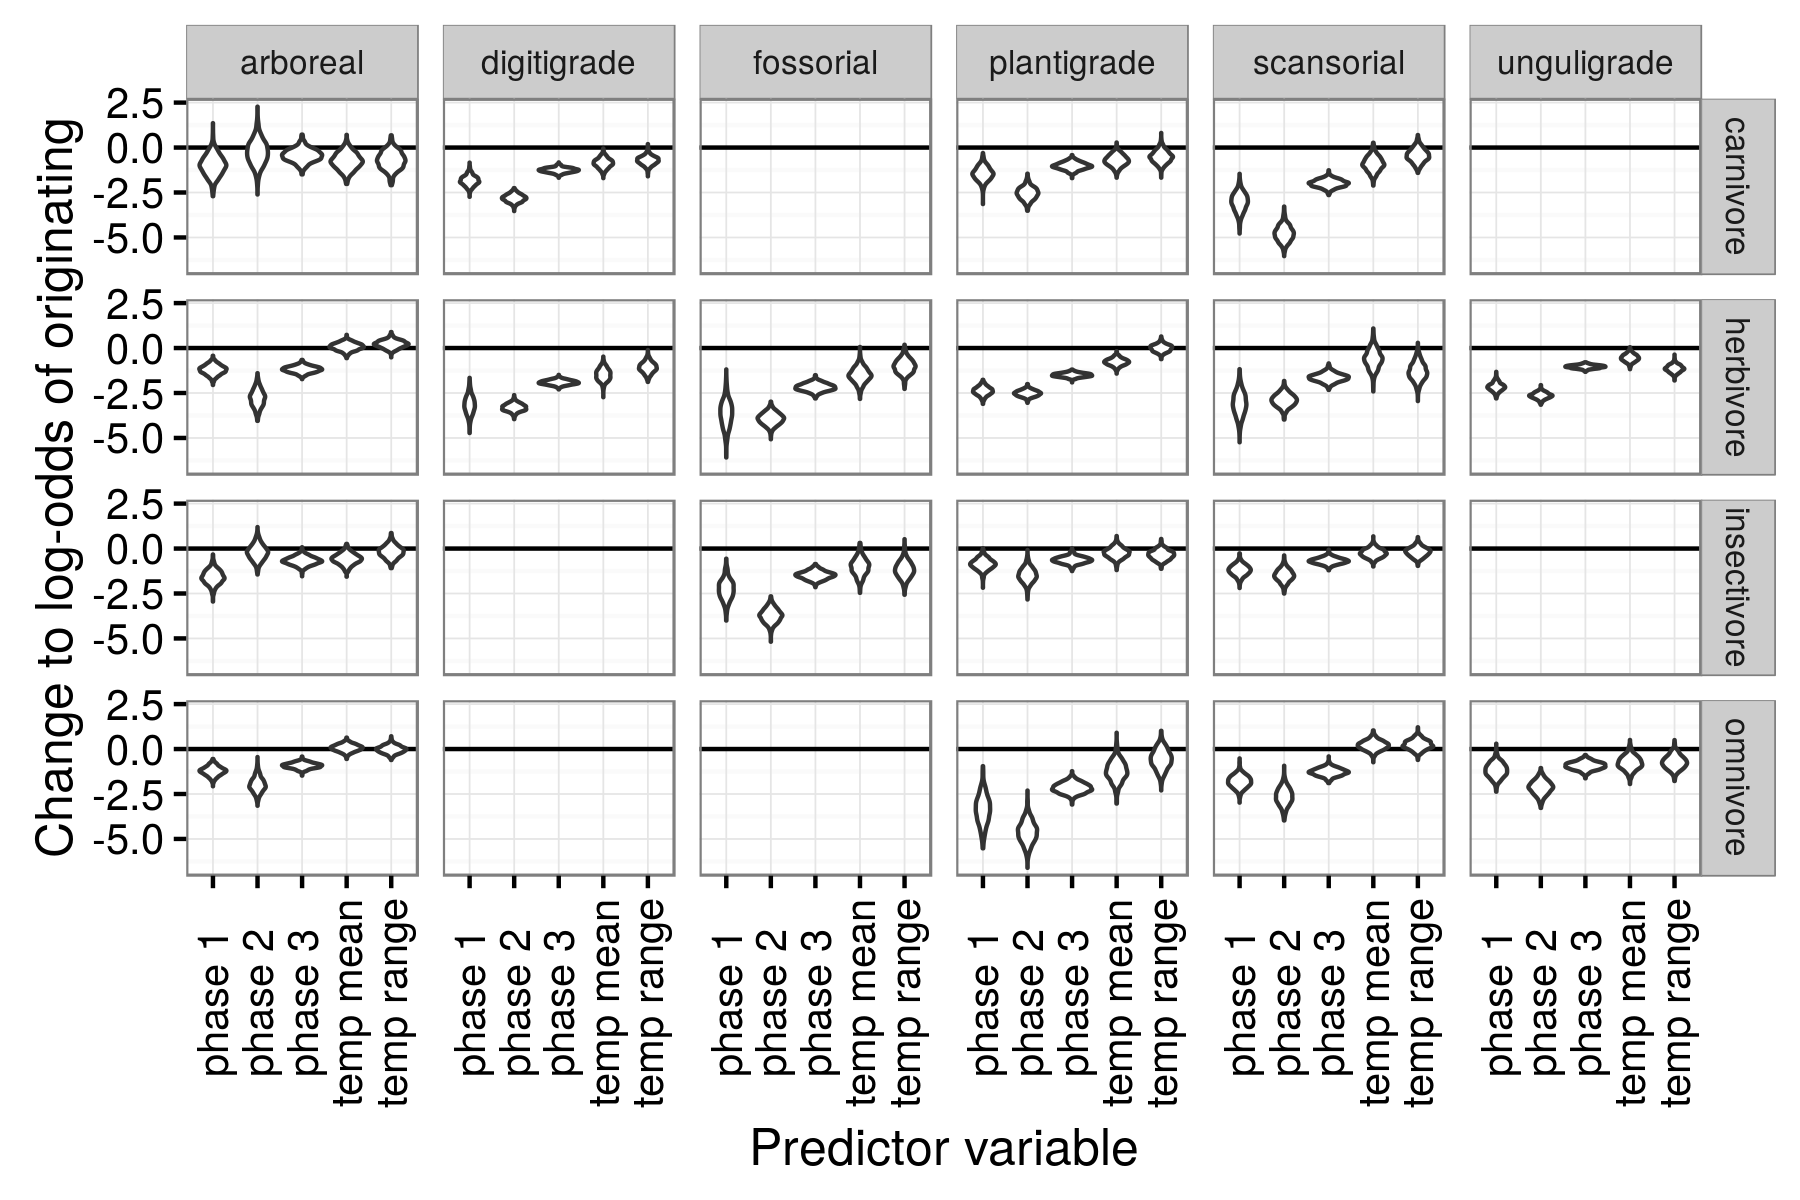
\includegraphics[width=\textwidth,height=0.4\textheight,keepaspectratio=true]{figure/group_on_origin_bd}
  \caption[Effects of group-level covariates on log-odds of ecotype origination as estimated from the birth-death model]{Estimated effects of the group-level covariates describing environmental context on log-odds of species origination. These estimates are from the birth-death model. What is plotted is a violin of the distribution of 1000 samples from the approximate posterior.} 
  \label{fig:group_origin_bd}
\end{figure}

% make these tables appendix
\begin{table}[ht]
  \centering
  \caption[Posterior probablity estimates of differences in origination by plant phase]{Posterior probability of the differences in the log-odds of an ecotype originating based on plant phase.} 
  \label{tab:origin_plant}
  \begin{tabular}{ l r r r }
    \hline
    & P(Eo.Mi $>$ 0) & P(Pa.Eo $>$ 0) & P(Eo.Mi $>$ Pa.Eo) \\ 
    \hline
    arboreal carnivore & 0.575 & 0.447 & 0.598 \\ 
    digitigrade carnivore & 0.976 & 0.017 & 0.998 \\ 
    plantigrade carnivore & 0.857 & 0.780 & 0.578 \\ 
    scansorial carnivore & 0.768 & 0.154 & 0.889 \\ 
    arboreal herbivore & 0.318 & 0.357 & 0.428 \\ 
    digitigrade herbivore & 1.000 & 0.161 & 0.995 \\ 
    fossorial herbivore & 0.999 & 0.353 & 0.926 \\ 
    plantigrade herbivore & 1.000 & 0.304 & 0.998 \\ 
    scansorial herbivore & 0.999 & 0.108 & 0.998 \\ 
    unguligrade herbivore & 0.000 & 0.000 & 0.100 \\ 
    arboreal insectivore & 0.364 & 0.003 & 0.857 \\ 
    fossorial insectivore & 0.645 & 0.341 & 0.708 \\ 
    plantigrade insectivore & 0.794 & 0.148 & 0.881 \\ 
    scansorial insectivore & 0.916 & 0.235 & 0.940 \\ 
    arboreal omnivore & 0.590 & 0.006 & 0.882 \\ 
    plantigrade omnivore & 0.524 & 0.209 & 0.762 \\ 
    scansorial omnivore & 0.713 & 0.027 & 0.938 \\ 
    unguligrade omnivore & 0.888 & 0.127 & 0.960 \\ 
    \hline
  \end{tabular}
\end{table}

\begin{table}[ht]
  \centering
  \caption[Posterior probablity of effects of temperature on origination]{Posterior probability that the effects of the two temperature covariates on the log-odds of an ecotype origination are greater than 0. What is estimated is the probability that these estimates are greater than 0; high or low probabilities indicate the ``strength'' of the covariate in that direction (positive and negative, respectively). These estimates are from the birth-death model.}
  \label{tab:origin_temp}
  \begin{tabular}{ l r }
    \hline
    & \(P(\gamma_{temp\ mean} > 0)\) \\
    \hline
    arboreal carnivore & 0.355 \\ 
    digitigrade carnivore & 0.001 \\ 
    plantigrade carnivore & 0.358 \\ 
    scansorial carnivore & 0.121 \\ 
    arboreal herbivore & 0.219 \\ 
    digitigrade herbivore & 0.045 \\ 
    fossorial herbivore & 0.067 \\ 
    plantigrade herbivore & 0.000 \\ 
    scansorial herbivore & 0.221 \\ 
    unguligrade herbivore & 0.339 \\ 
    arboreal insectivore & 0.027 \\ 
    fossorial insectivore & 0.219 \\ 
    plantigrade insectivore & 0.224 \\ 
    scansorial insectivore & 0.192 \\ 
    arboreal omnivore & 0.009 \\ 
    plantigrade omnivore & 0.087 \\ 
    scansorial omnivore & 0.035 \\ 
    unguligrade omnivore & 0.129 \\ 
    \hline
  \end{tabular}
\end{table}

%     correlation
None of the time-series of functional group origination probability are estimated to be either positively or negatively correlated (Fig. \ref{fig:origin_corr}). This result indicates that functional groups have independent origination histories for the Cenozoic. This result does not preclude the possibility of short term similiarities in expansion and decline of orgination probability or shared peaks and troughs of origination probability. Additionally, if the relationship between two functional groups changes over time (e.g. from positive correlation to negative correlation), then it woud yield no overall correlation for the Cenozoic. Finally, it is important to remember that this estimate correlation is based on origination probability and not origination rate or diversity.
\begin{figure}[ht]
  \centering
  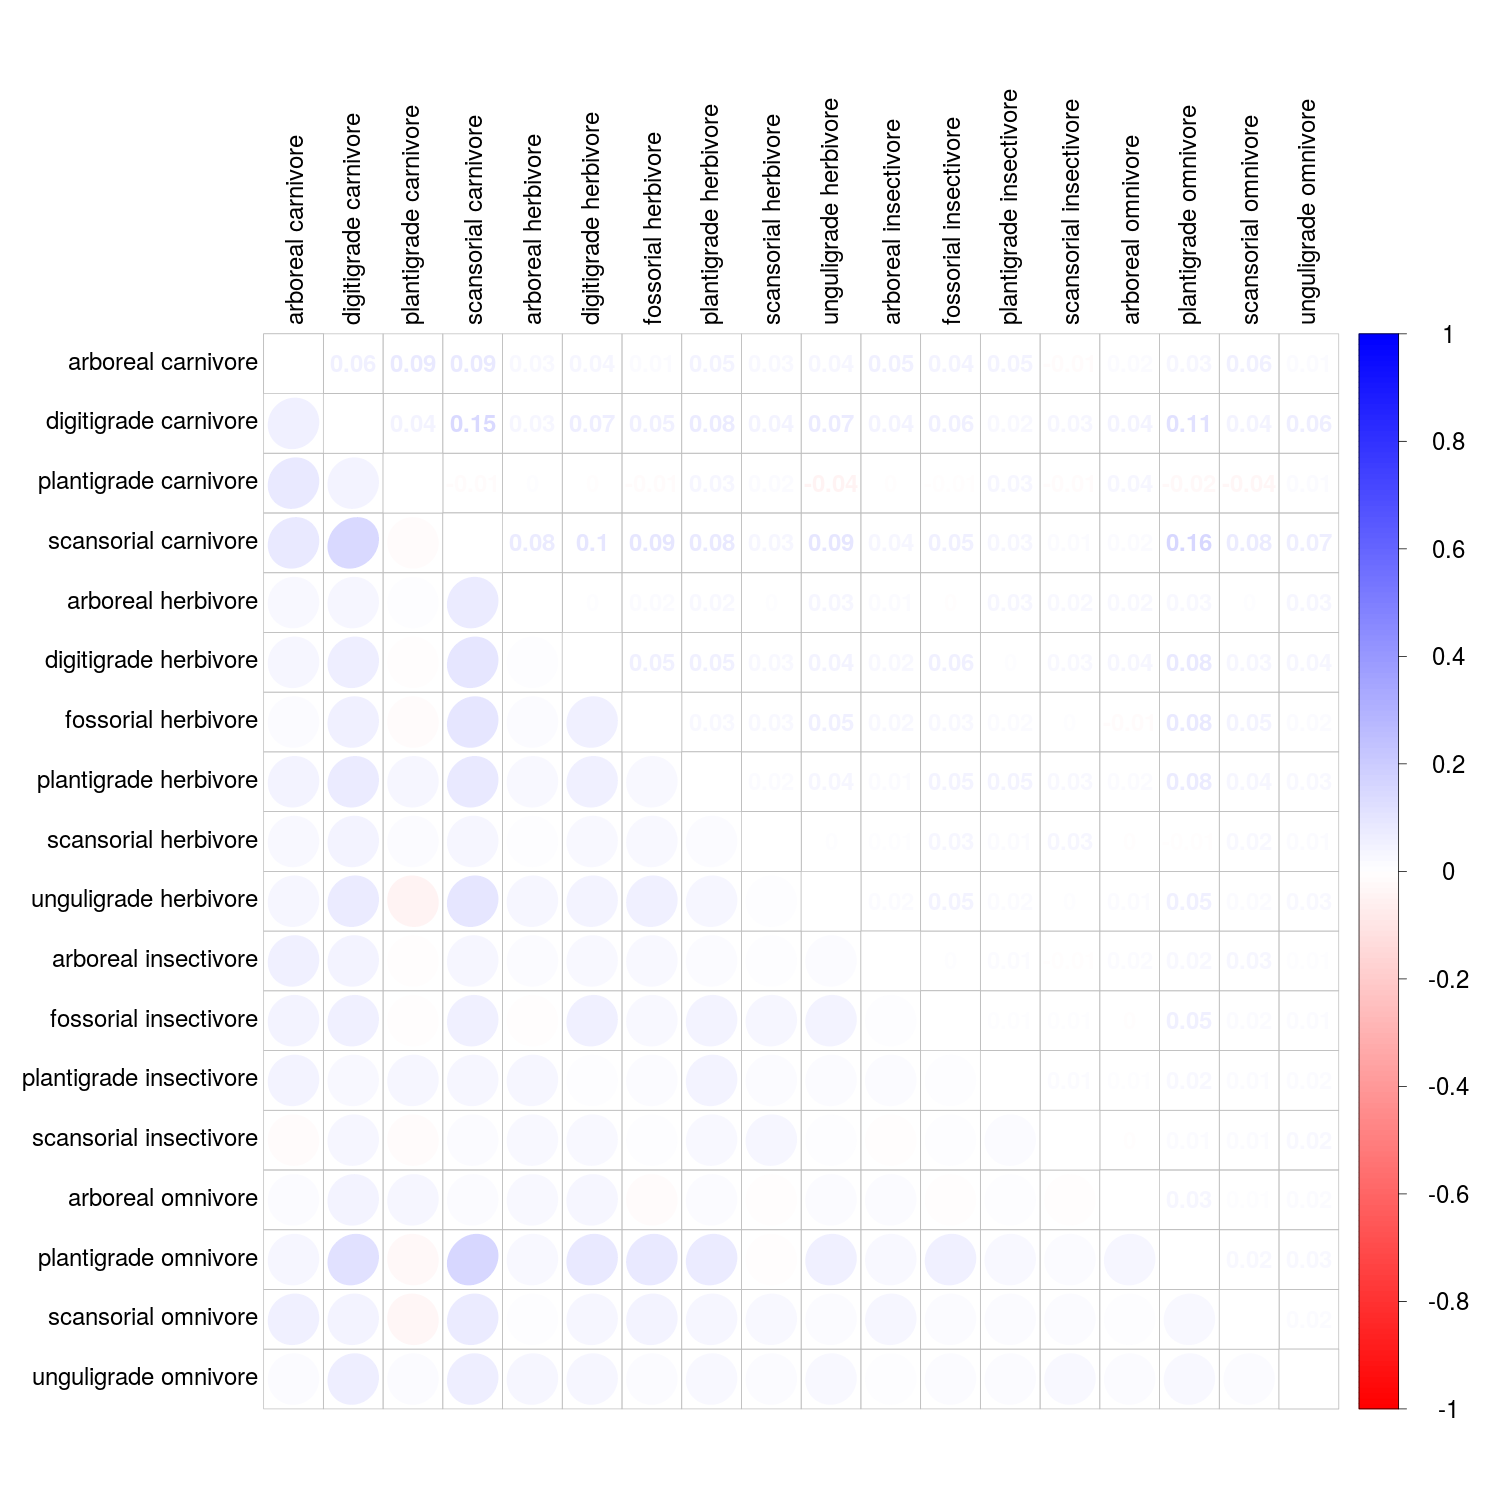
\includegraphics[width=\textwidth,height=\textheight,keepaspectratio=true]{figure/origination_correlation}
  \caption[Estimated correlations in origination probability between ecotypes]{Posterior mean estimates of the correlations in origination probability between the mammal ecotypes. The lower triangle of the matrix is populated with ellipses corresponding to the level of correlation between the two ecotypes, while the upper triangle of the matrix corresponds to the mean estimated correlation between ecotypes. Darker values correspond to a greater magnitude of correlation with blue values corresponding to a positive correlation and red values a negative correlation.}
  \label{fig:origin_corr}
\end{figure}





% survival
%   individual-level
%     FG time series
The survival probability time-series vary greatly between each of the functional groups with each exhibiting unique patterns (Fig. \ref{fig:eco_survival}). Interestingly, unlike origination probability (Fig. \ref{fig:eco_origin}), survival probability is frequently estimated estimated with considerable uncertainty. When survival probability is below 0.50 then a species that is present is unlikely to survive from one time unit to the next, while when survival probability is greater than 0.50 species can be expected to survive to the next time unit. Finally, when survival probability is approximately 0.50 then survival and extinction are equally likely. Overall, survival probability is rarely estimated to be greater than 0.50 with any certainty. This result is consistent with the average occurrence being \(<\)1.35 time unit per species which means that a plurality of species have only a single temporal occurrence (Fig. \ref{fig:ppc}).

The survival probability of many functional groups is frequently approximately 0.50, indicating extinction is frequently random with respect to functional group (Fig. \ref{fig:eco_survival}). For example, the survival probability scansorial canirvores is approximately 0.50 for the entire time series which indicates that there is no best or worst time for this functional groups survival. Similar patterns can be observed for mean survival probability of arboreal omnivores, fossorial insectivores, and plantigrade omnivores though all three of these groups have sudden drops in survival probability in approximately the last 10Mya.

Arboreal herbivores are the only functional group for which survival probability is approximately above 0.50 for the entire Cenozoic (Fig. \ref{fig:eco_survival}). This result indicates that when an arboreal herbivore species is present it is expected to survive from one time unit to the next. However, it is important to note that arboreal herbivores are estimated to have an origination probability below 0.50 for most of the Cenozoic. Together, these results mean that arboreal herbivore species are rare but are expected to survive from one time point to the next.

A common feature of multiple functional group's survival probability time-series is a peak in survival during the Neogene (Fig. \ref{fig:eco_survival}). In most cases, these peaks are estimated with little uncertainty which indicates how apparent this event is. Digitigrade carnivores, digitigrade herbivores, plantigrade herbivores, scansorial insectivores, unguligrade herbivores, and unguligrade omnivores all peak in survival probability at approximately 25Mya. This peak in survival means that species of these functional groups which are unlikely to go extinct at this point, potentially indicating favorable environmental conditions for these groups at the Paleogene-Neogene transition. Additionally, this peak does not coincide with the movement from one plant phase to another (Table \ref{tab:plant_def}). 
\begin{figure}[ht]
  \centering
  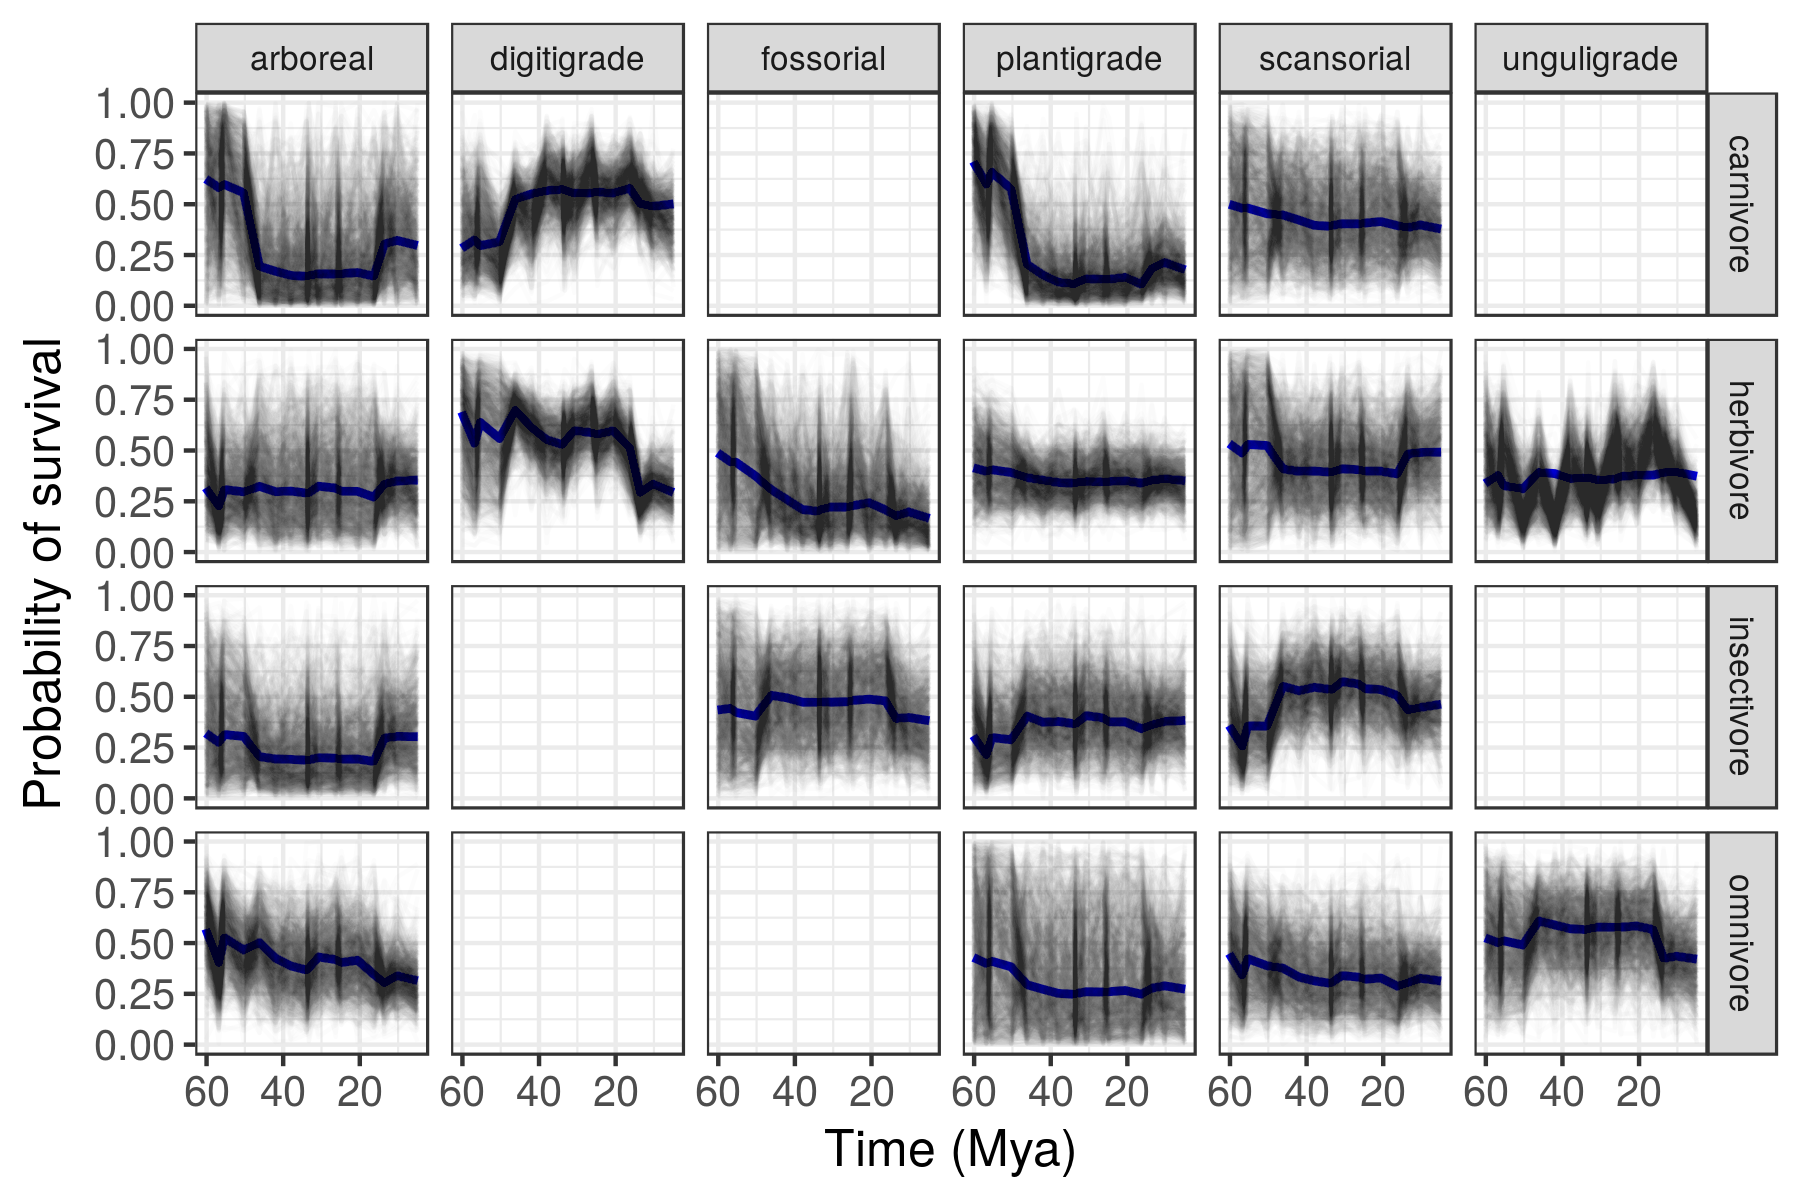
\includegraphics[width=\textwidth,height=0.4\textheight,keepaspectratio=true]{figure/ecotype_survival_bd}
  \caption[Ecotype survival probability estimated from the birth-death model]{Probability of a mammal ecotype survival probabilities at each time point as estimated from the birth-death model. Each panel depicts 100 random samples from the model's posterior. The columns are by locomotor category and rows by dietary category; their intersections are the observed and analyzed ecotypes. Panels with no lines are ecotypes not observed in the dataset.}
  \label{fig:eco_survival}
\end{figure}

%     order effect
The effect of order on survival probability has much lower variance (Fig. \ref{fig:order_surv}) than the effect of order on origination probability (Fig. \ref{fig:order_origin}. Primates, Multituberculata, Eulipotyphla, Dermoptera, Creodonta, Condylarthra, Carnivora, and Artiodactyla are estimated to have a lower than average survival probability which implies that species of these orders are expected to be present for a single time unit. Of these orders, Primates and Multituberculata are expected to have the lowest survival probability of all orders. The orders expected to have greater than average survival probability are Rodentia, Lagomorpha, and Didelphimorphia.
\begin{figure}[ht]
  \centering
  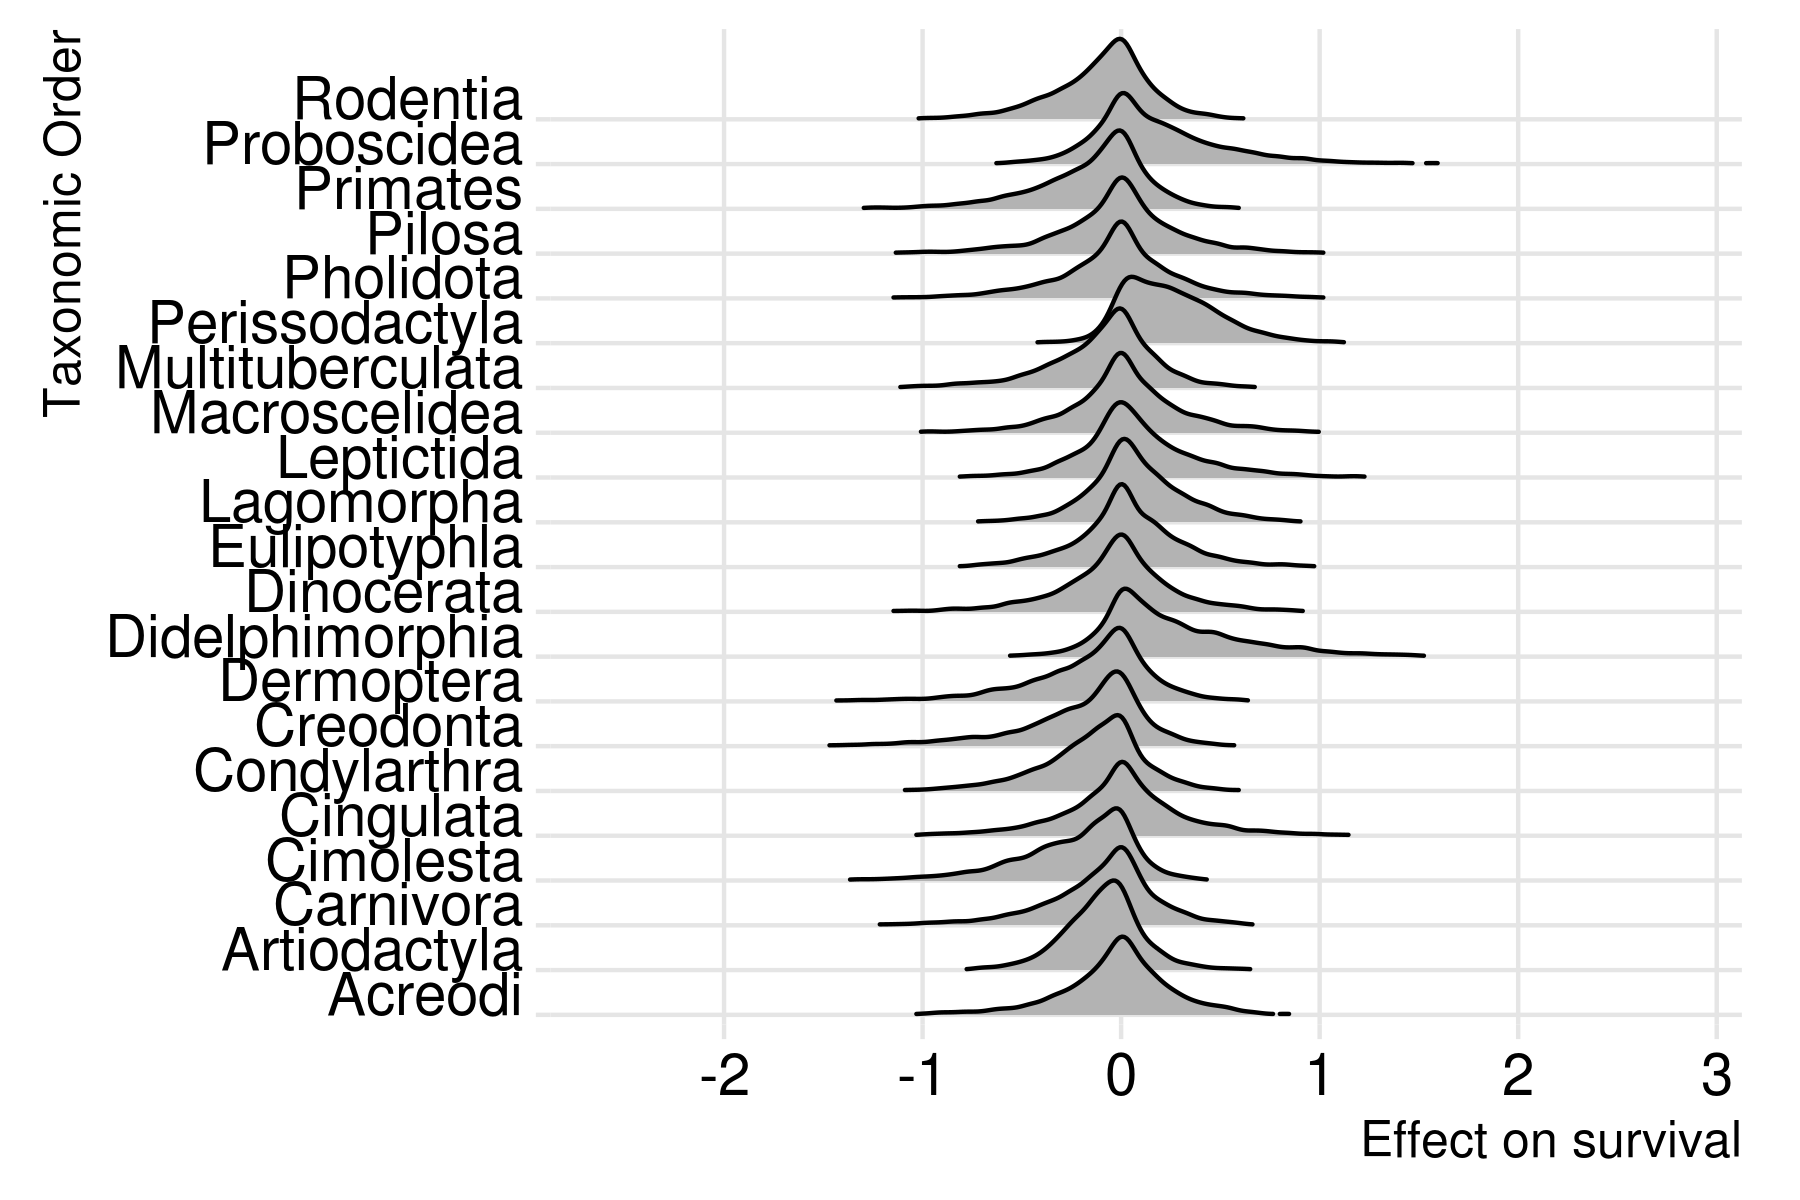
\includegraphics[width=\textwidth,height=0.4\textheight,keepaspectratio=true]{figure/order_survival_bd}
  \caption{Differences in log-odds of survival based on mammal orders. Positive values correspond to greater log-odds of survival than average, while negative values correspond to lower log-odds of survival than average.}
  \label{fig:order_surv}
\end{figure}

%     mass effect
Species mass is estimated to have no relationship or at best a weakly positive relationship with survival probability (Fig. \ref{fig:mass_survival}). This result means that differences in mass do not lead to differences in species survival. This result is consistent with previous studies of North American species and genus survival dynamics CITATION SMITS TOMIYA, and implies that other ecological factors have greater importance on survival than mass alone. \uppercase{get probability estimate}
\begin{figure}[ht]
  \centering
  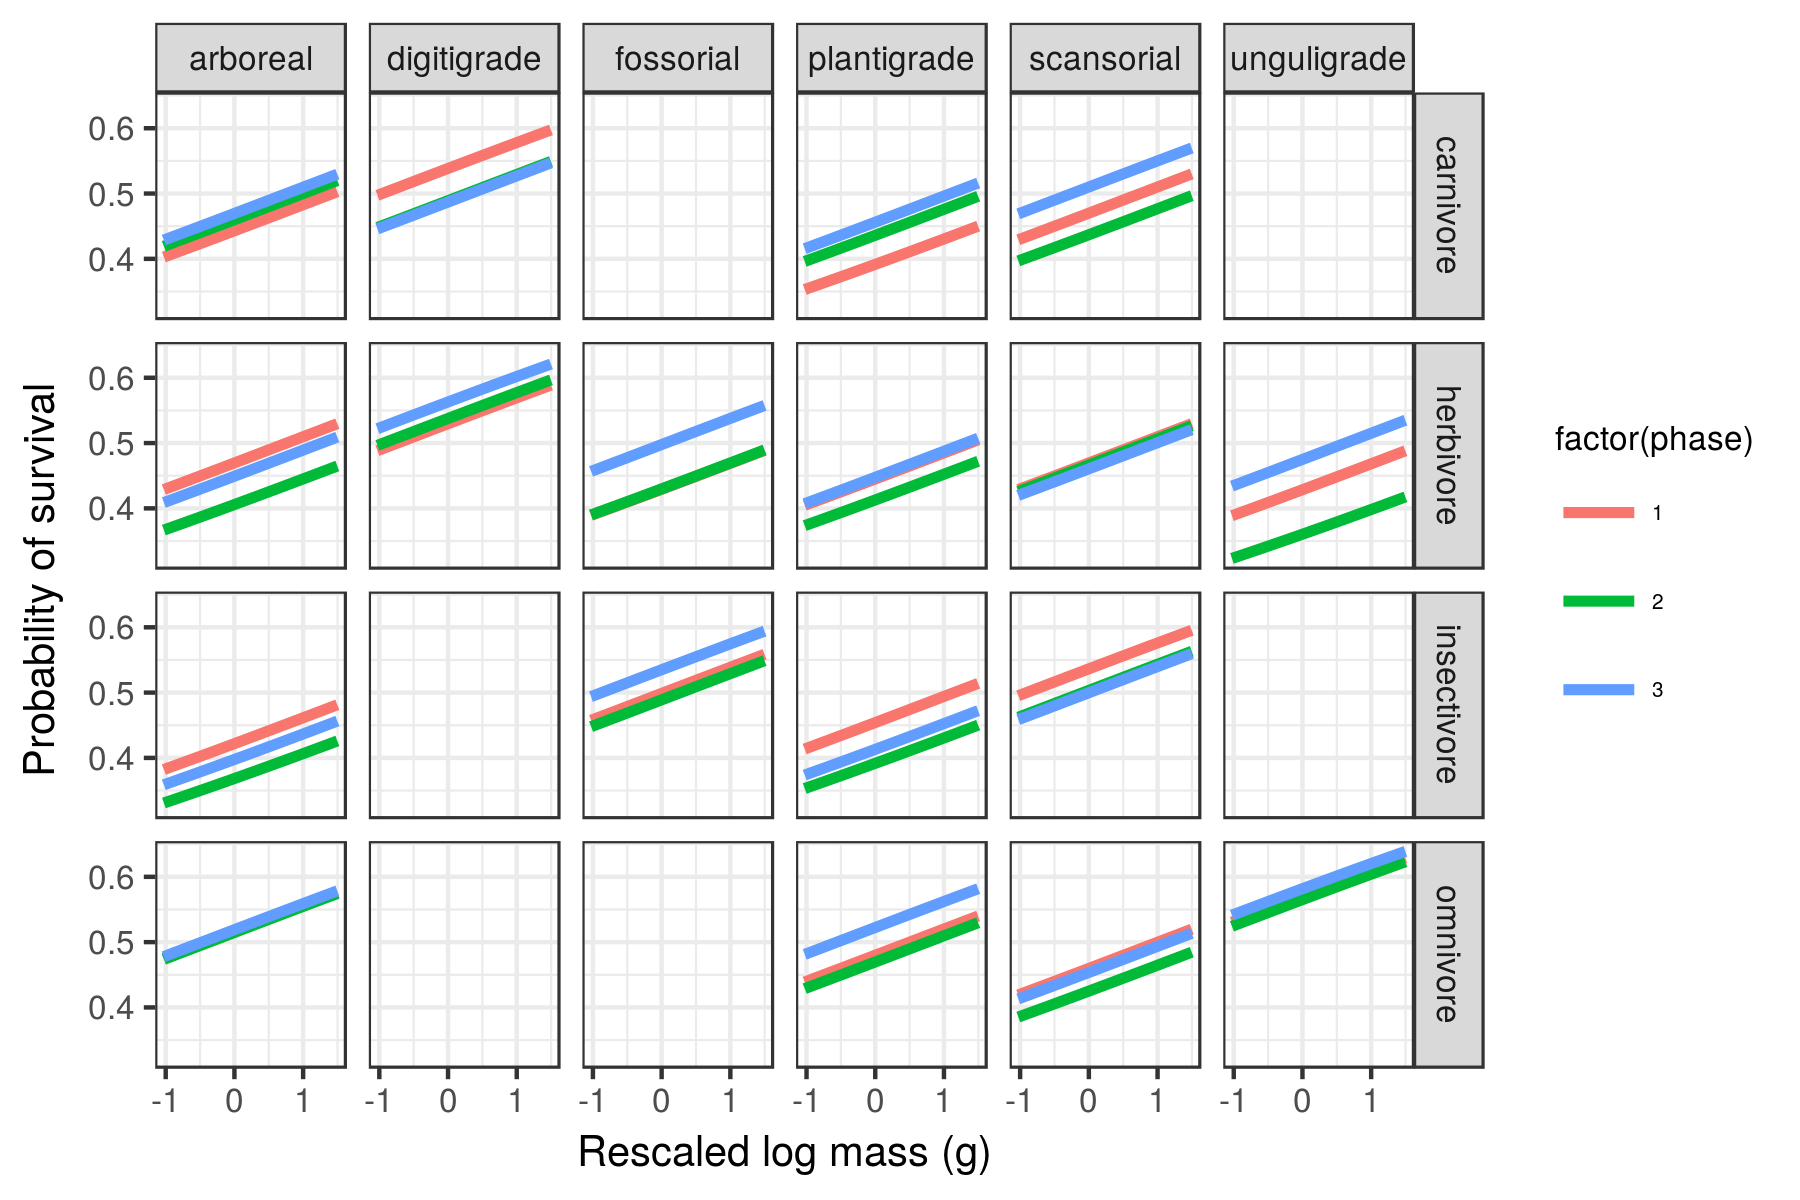
\includegraphics[width=\textwidth,height=0.4\textheight,keepaspectratio=true]{figure/mass_on_surv_bd}
  \caption[Effect of mass on probability of species survival as estimated from the birth-death model]{Mean estimate of the effect of species mass on the probability of a species survival for each of the three plant phases. The effect of mass is considered constant over time and that the only aspect of the model that changes with plant phase is the intercept of the relationship between mass and survival. The three plant phases are indicated by the color of the line. Mass has been log-transformed, centered, and rescaled; this means that a mass of 0 corresponds to the mean of log-mass of all observed species and that mass is in standard deviation units. For clarity, only the mean estimates of the effects of mass and plant plant are plotted.}
  \label{fig:mass_survival}
\end{figure}

%   group-level
%     temperature and plant phase
In contrast to the origination probability, there is little evidence that the group-level covariates have large effects on functional group survival probabilities (Fig. \ref{fig:group_surv_bd}). In fact, only the plant phases are associated with differences in survival probability and only for a relatively small number of functional groups. These results combined with those from the individual-level covariates (Fig. \ref{fig:eco_survival}, \ref{fig:order_surv}, \ref{fig:mass_survival}) imply that direct interactions (e.g. species--species) are potentially more important to long term species survival than ambient environemnt (e.g. temperature tolerance). However, because this estimate of temperature is global in nature, this interpretation is inherently speculative.

Functional group survival probability is rarely associated with differences between the three plant phases (Table \ref{tab:surv_plant}) with only five pair-wise comparisons having greater than 89\% probability of differences in survival between phases. Unuligrade herbivores have an approximately 89\% probability of having lower survival probability during the Paleocene-Eocene than the Miocene-Pleistocene. For digitgrade herbivores, and unguligrade ominvores, the Eocene-Miocene phase have an approximately 90\% probability of having greater survival probability than during the Micocene-Pleistocene phase. In contrast, unguligrade herbivores are estimated to have lower survival probability in the Eocene-Miocene phase than the Miocene-Pleistocene phase. Finally, unguligrade herbivores have an approximately 99\% probability of having a lower survival probability during the Paleocene-Eocene than the Eocene-Miocene.

As stated earlier, temperature is estimated to have no effect on functional group survival probability (Table \ref{tab:surv_temp}). This is congruent with previous studies which found no association between extinction and global temperature CITATION ALROY or no consistent, unidirectional relationship between extinction and global temperature CITATION. 

\begin{figure}[ht]
  \centering
  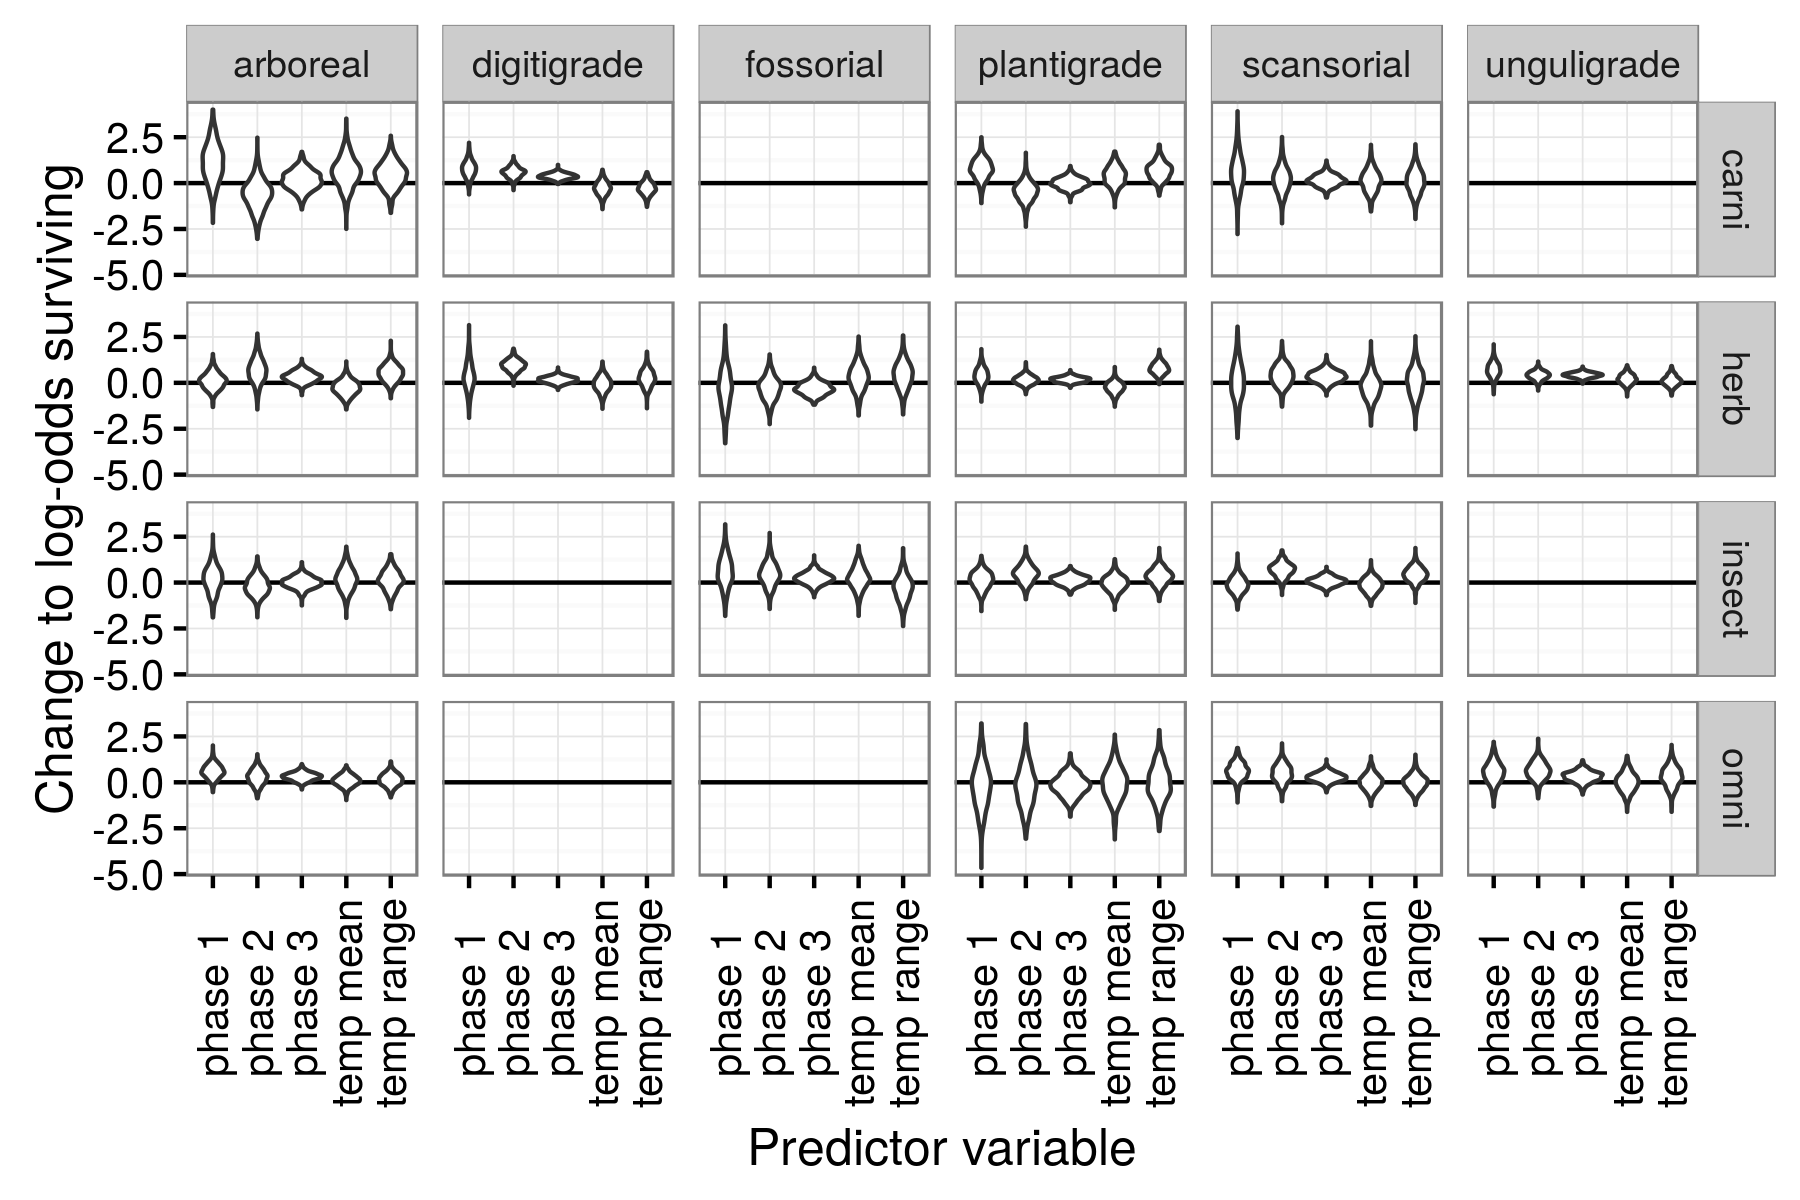
\includegraphics[width=\textwidth,height=0.4\textheight,keepaspectratio=true]{figure/group_on_survival_bd}
  \caption[Effects of group-level covariates on log-odds of ecotype survival as estimated from the birth-death model]{Estimated effects of the group-level covariates describing environmental context on log-odds of species survival. These estimates are from the birth-death model. What is plotted is a violin of the distribution of 1000 samples from the approximate posterior.}
  \label{fig:group_surv_bd}
\end{figure}

% make these tables appendix
\begin{table}[ht]
  \centering
  \caption[Posterior probablity estimates of differences in survival by plant phase]{Posterior probability of the differences in the log-odds of an ecotype surviving based on plant phase.} 
  \label{tab:surv_plant}
  \begin{tabular}{ l r r r }
    \hline
    & P(Eo.Mi $>$ 0) & P(Pa.Eo $>$ 0) & P(Eo.Mi $>$ Pa.Eo) \\ 
    \hline
    arboreal carnivore & 0.297 & 0.560 & 0.328 \\ 
    digitigrade carnivore & 0.786 & 0.367 & 0.743 \\ 
    plantigrade carnivore & 0.411 & 0.744 & 0.273 \\ 
    scansorial carnivore & 0.428 & 0.445 & 0.486 \\ 
    arboreal herbivore & 0.256 & 0.768 & 0.174 \\ 
    digitigrade herbivore & 1.000 & 0.400 & 0.942 \\ 
    fossorial herbivore & 0.696 & 0.563 & 0.565 \\ 
    plantigrade herbivore & 0.659 & 0.508 & 0.596 \\ 
    scansorial herbivore & 0.616 & 0.539 & 0.531 \\ 
    unguligrade herbivore & 0.000 & 0.102 & 0.012 \\ 
    arboreal insectivore & 0.289 & 0.483 & 0.368 \\ 
    fossorial insectivore & 0.532 & 0.420 & 0.592 \\ 
    plantigrade insectivore & 0.499 & 0.361 & 0.605 \\ 
    scansorial insectivore & 0.443 & 0.252 & 0.634 \\ 
    arboreal omnivore & 0.651 & 0.597 & 0.591 \\ 
    plantigrade omnivore & 0.417 & 0.549 & 0.393 \\ 
    scansorial omnivore & 0.486 & 0.525 & 0.487 \\ 
    unguligrade omnivore & 0.929 & 0.521 & 0.844 \\ 
    \hline
  \end{tabular}
\end{table}

\begin{table}[ht]
  \centering
  \caption[Posterior probablity of effects of temperature on survival]{Posterior probability that the effects of the two temperature covariates on the log-odds of an ecotype survival are greater than 0. What is estimated is the probability that these estimates are greater than 0; high or low probabilities indicate the ``strength'' of the covariate in that direction (positive and negative, respectively). These estimates are from the birth-death model.}
  \label{tab:surv_temp}
  \begin{tabular}{ l r r }
    \hline
    & \(P(\gamma_{temp\ mean} > 0)\) \\
    \hline
    arboreal carnivore & 0.665 \\ 
    digitigrade carnivore & 0.453 \\ 
    plantigrade carnivore & 0.618 \\ 
    scansorial carnivore & 0.380 \\ 
    arboreal herbivore & 0.761 \\ 
    digitigrade herbivore & 0.395 \\ 
    fossorial herbivore & 0.429 \\ 
    plantigrade herbivore & 0.279 \\ 
    scansorial herbivore & 0.345 \\ 
    unguligrade herbivore & 0.818 \\ 
    arboreal insectivore & 0.489 \\ 
    fossorial insectivore & 0.452 \\ 
    plantigrade insectivore & 0.435 \\ 
    scansorial insectivore & 0.384 \\ 
    arboreal omnivore & 0.600 \\ 
    plantigrade omnivore & 0.639 \\ 
    scansorial omnivore & 0.512 \\ 
    unguligrade omnivore & 0.396 \\ 
    \hline
  \end{tabular}
\end{table}

%     correlation
None of the time-series of functional group survival probability are estimated to be either positively or negatively correlated (Fig. \ref{fig:survival_corr}); this mirrors the correlations in origination probabliity (Fig. \ref{fig:origin_corr}). This result indicates that functional groups probably have independent survival histories for the Cenozoic. As with origination probability, this result does not preclude the possibility of short term similiarities in expansion and decline of orgination probability or shared peaks and troughs of survival probability. Additionally, if the relationship between two functional groups changes over time (e.g. from positive correlation to negative correlation), then it woud yield no overall correlation for the Cenozoic. Finally, it is important to remember that this estimate correlation is based on survival probability and not extinction rate or diversity.
\begin{figure}[ht]
  \centering
  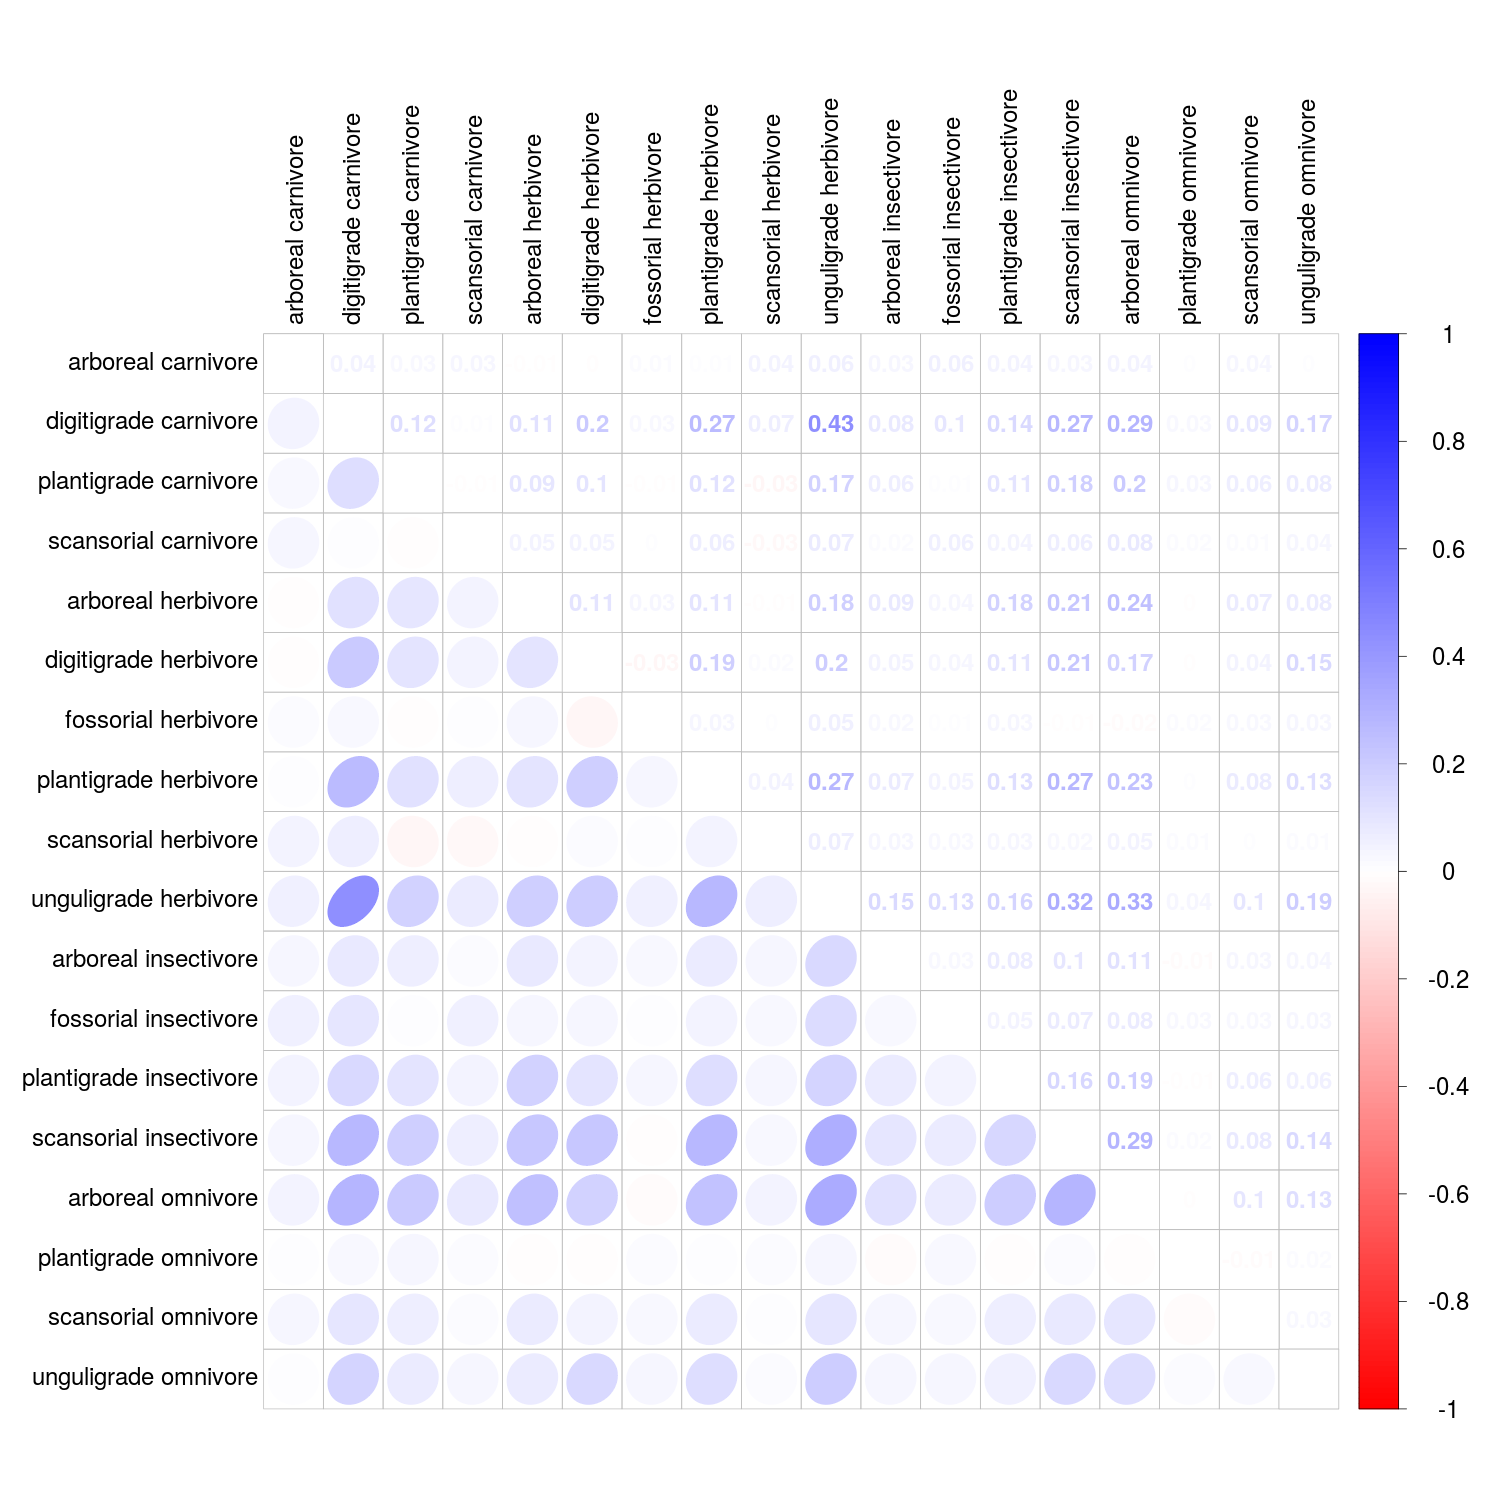
\includegraphics[width=\textwidth,height=\textheight,keepaspectratio=true]{figure/survival_correlation}
  \caption[Estimated correlations in survival probability between ecotypes]{Posterior mean estimates of the correlations in survival probability between the mammal ecotypes. The lower triangle of the matrix is populated with ellipses corresponding to the level of correlation between the two ecotypes, while the upper triangle of the matrix corresponds to the mean estimated correlation between ecotypes. Darker values correspond to a greater magnitude of correlation with blue values corresponding to a positive correlation and red values a negative correlation.}
  \label{fig:survival_corr}
\end{figure}







\subsection*{Analysis of diversity}
Standing diversity of the North American mammal species pool estimated from this model exhibits an initial increase in diversity followed by a slow decrease till approximately 30Mya, afterwhich there is a marked increase till approximately 15Mya after which it decreases slightly till it is equal to the overall mean diversity of the Cenozoic (Fig. \ref{fig:diversity_est}). Per-unit standing diveristy is found to be different from average standing diversity for 12 of 18 time-units (\(> 85\) probability; Table \ref{tab:div_peak}). Diversity is greater than average during the Tiffanian, Wasatchian, Hemingfordian, Barsotvian, and Clarendonian while diversity is lower than average during the Duchesnean, Chadronian, Orellan, Whitneyan, Geringian, Monroecreekian, and Harrisonian. The nadir of diversity is the Orellan while the apex is the Barstovian (Fig. \ref{fig:diversity_est}). Interstingly, the rise in diversity among the sampled species from the Orellan to the Barstovian is unidirectional and is not estimated to have any temporary dips in diversification for that entire approximately 15 million year period.
\begin{figure}[ht]
  \centering
  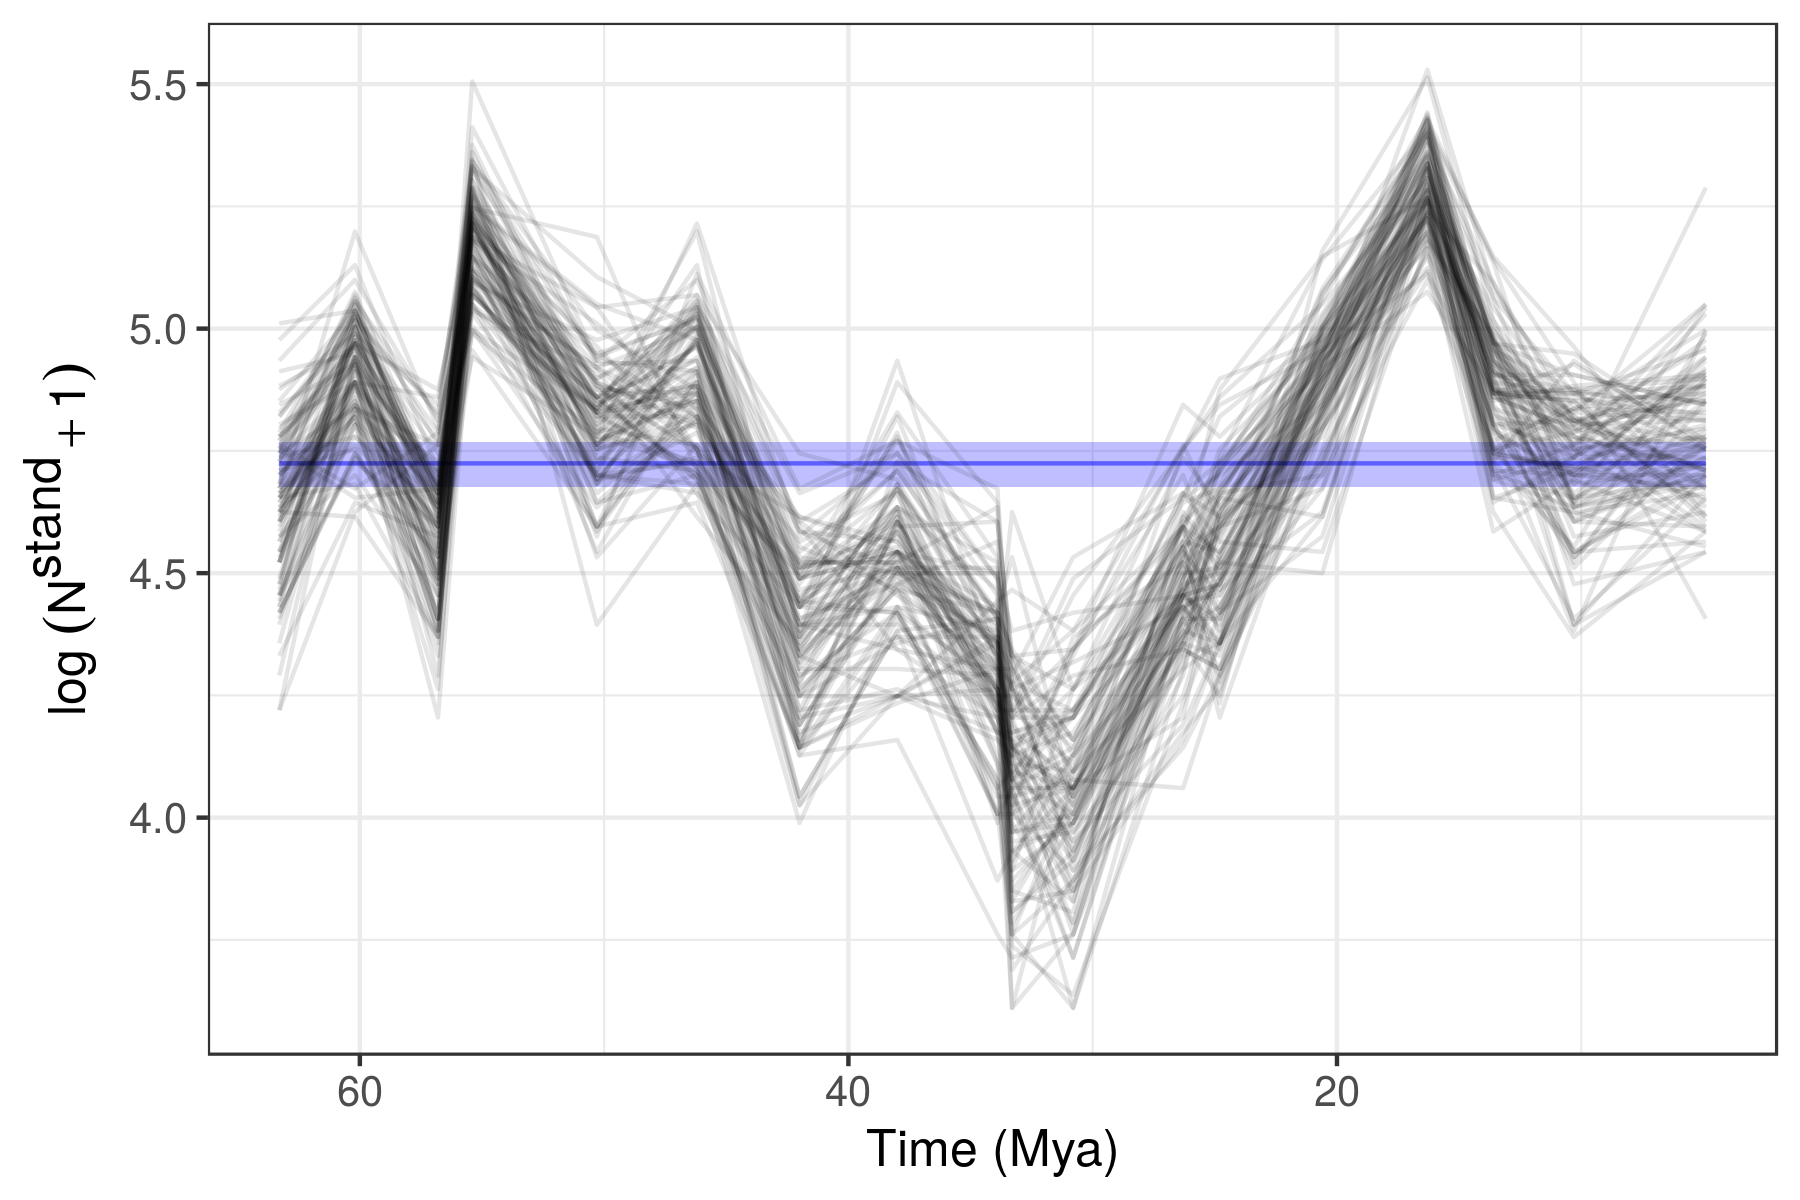
\includegraphics[width=\textwidth,height=0.5\textheight,keepaspectratio=true]{figure/log_diversity}
  \caption{Log diversity}
  \caption[Estimated mammal log-diversity for the Cenozoic]{Posterior estimates of the time series of Cenozoic North American mammal diversity; all estimates are from 100 posterior draws. The blue horizontal strip corresponds to the median and 80\% credible interval of estimated mean standing diversity.} 
  \label{fig:diversity_est}
\end{figure}

\begin{table}[ht]
  \centering
  \caption[Posterior probability estimates of a peak in diversity]{Posterior probabilities of diversity \(N^{stand}_{t}\) greater than average standing diversity \(\overline{N^{stand}}\) for the whole Cenozoic. The NALMA column corresponds to North American Land Mammal age for that estimate.}
  \label{tab:div_peak}
  \begin{tabular}{ r r }
    \hline
    NALMA & \(P(N^{stand}_{t} > \overline{N^{stand}})\) \\
    \hline
    Torrejonian & 0.79 \\ 
    Tiffanian & 0.95 \\ 
    Clarkforkian & 0.50 \\ 
    Wasatchian & 1.00 \\ 
    Bridgerian & 0.69 \\ 
    Uintan & 0.75 \\ 
    Duchesnean & 0.00 \\ 
    Chadronian & 0.01 \\ 
    Orellan & 0.00 \\ 
    Whitneyan & 0.00 \\ 
    Geringian & 0.00 \\ 
    Monroecreekian & 0.01 \\ 
    Harrisonian & 0.11 \\ 
    Hemingfordian & 0.96 \\ 
    Barstovian & 1.00 \\ 
    Clarendonian & 0.93 \\ 
    Hemphillian & 0.63 \\ 
    Blancan & 0.73 \\ 
    \hline
  \end{tabular}
\end{table}


Standing diversity when partitioned by ecotype reveals a lot of the complexity behind the pattern of mammal diversity for the Cenozoic (Fig. \ref{fig:ecotype_diversity}). While each functional group has its own unique diveristy history, there are some broad similarities as is similar to the estimates origination and survival probability (Fig. \ref{fig:eco_origin}, \ref{fig:eco_survival}).

Arboreal ecotypes obtain peak diversity early in the Cenozoic and then decline for the rest of the time series, becoming increasingly rare or absent as diversity approaches the Recent (Fig. \ref{fig:ecotype_diversity}). Arboreal herbivores and omnivores obtain peak diversity at the beginning of the Cenozoic then go into decline while remaining a small part of the species pool, while arboreal carnivores and insectivores obtain peak diversity approximately 55 Mya and then quickly decline and become extremely rare or entirely absent from the species pool. The only arboreal functional group estimated to not experience a complete disappearance from the species pool are arboreal herbivores. This is consistent with increasing extinction risk in the Neogene compared to the Paleogene as proposed by \citet{Smits2015b}.

The diversity of plantigrade insectivores, scansorial insectivores, and scansorial omnivores are estimated to decrease through the Cenozoic (Fig. \ref{fig:ecotype_diversity}). Plantigrade herbivores and scansorial omnivores have peak diversity at the early Cenozoic and reach low diversity by 30Mya, after which diversity never increases again. In contrast, scansorial omnivores have nearly constant, above average diversity for the beginning of the Cenozoic till approximately 30Mya, after which diversity drops and remaining below average diversity for the rest of the Cenozoic.

The fossorial functional groups included in this study are estimated to be rare or absent absent for the first half of the Cenozoic, fossorial herbivores probably having lower diversity than fossorial insectivores (Fig. \ref{fig:ecotype_diversity}). After fossorial herbivores increase in diversity approximately 30Mya, this functional group is estimated to quickly reach approximately constant standing diversity for the rest of the Cenozoic. In contrast, fossorial insectivores increase in diversity starting approximately 30Mya and reach max diversity approximately 15Mya, after which this group declines in diversity.

Plantigrade carnivores, scansorial herbivores and unguligrade omnivores are estimated to maintain near constant standing diversity for most of the Cenozoic (Fig. \ref{fig:ecotype_diversity}). Of these three functional groups, plantigrade carnivores have the greatest variance in standing diversity. Plantigrade carnivores have greater than average standing diversity from the beginning of the Cenozoic till 50Mya and from approximately 25Mya till approximately 15Mya. This functional group is estimated to be below average standing diversity from 50Mya to 30Mya, and then from 10Mya till the end of the studied time period. Scansorial herbivores exhibit a similar patterns but with a reversed diversity pattern for the first 30My of the studied period. Instead of near constant diversity, scansorial herbivores are estimated to have lower than average diversity from the beginning of the Cenozoic till approximately 50Mya, after which this group has approximately average standing diversity for the rest of the Cenozoic. The unguligrade omnivore functional group has slightly elevated diversity at the beginning of the Cenozoic and a possible decrease in diversity approximately 15Mya. 

Scansorial carnivores and plantigrade herbivores have below average standing diversity from the beginning of the Cenozoic till approximately 20Mya, after which both functional groups increase in diversity till being well above average by the end of the study period (Fig. \ref{fig:ecotype_diversity}). Plantigrade omnivores are estimated to be absent or extremely rare in the species pool, only increasing in standing diversity beginning approximately 25Mya. In contrast, scansorial carnivores are estimated to have been a rare but constant part of the species pool diversity for the entire Cenozoic with an increase in standing diversity starting approximately 25Mya.

Digitigrade carnivores, plantigrade herbivores, and unguligrade herbivores functional groups maintain relatively high standing diversity through out the entire Cenozoic though each exhibits periods of greater than average and below average standing diversity (Fig. \ref{fig:ecotype_diversity}). Digitigrade carnivore diversity is estimated to begin the study period below average and then quickly rise to the first peak in diversity at approximately 55Mya. After this, ditigrade carnivore diversity decreases to below average diversity till approximately 35Mya, after which diversity increases till a second greater peak in diversity approximately 15Mya. After this second peak in diversity, ditigrade carnivore diversity declines until the end of the study period. Unguligrade herbivores exhibit a similar pattern though with considerably less uncertainty. In contrast, while plantigrade herbivores have a similar increase and peak in diversity during the first half of the Cenozoic, the functional group does not experience a second peak in functional diversity till the end of the study period. Additionally, plantigrade herbivores have a longer period of above average standing diveristy during the first half of the Cenozoic, only experiencing a marked decrease in diversity starting approximately 35Mya.

The digitigrade herbivore functional group is estimated to be the only group with a near constant increase in standing diversity through most of the Cenozoic (Fig. \ref{fig:ecotype_diversity}). There are two periods of decrease in the standing diversity of digitigrade herbivores: the first approximately 10My of the study period, and a sudden decrease at 15Mya. Beyond these two decreases, this functional group exhibits a remarkable increase in diversity from relative rarity approximately 50-55My till peak diversity 15-20Mya. Diversity even appears to begin to rebound after the sudden decrease approximately 15Mya.
\begin{figure}[ht]
  \centering
  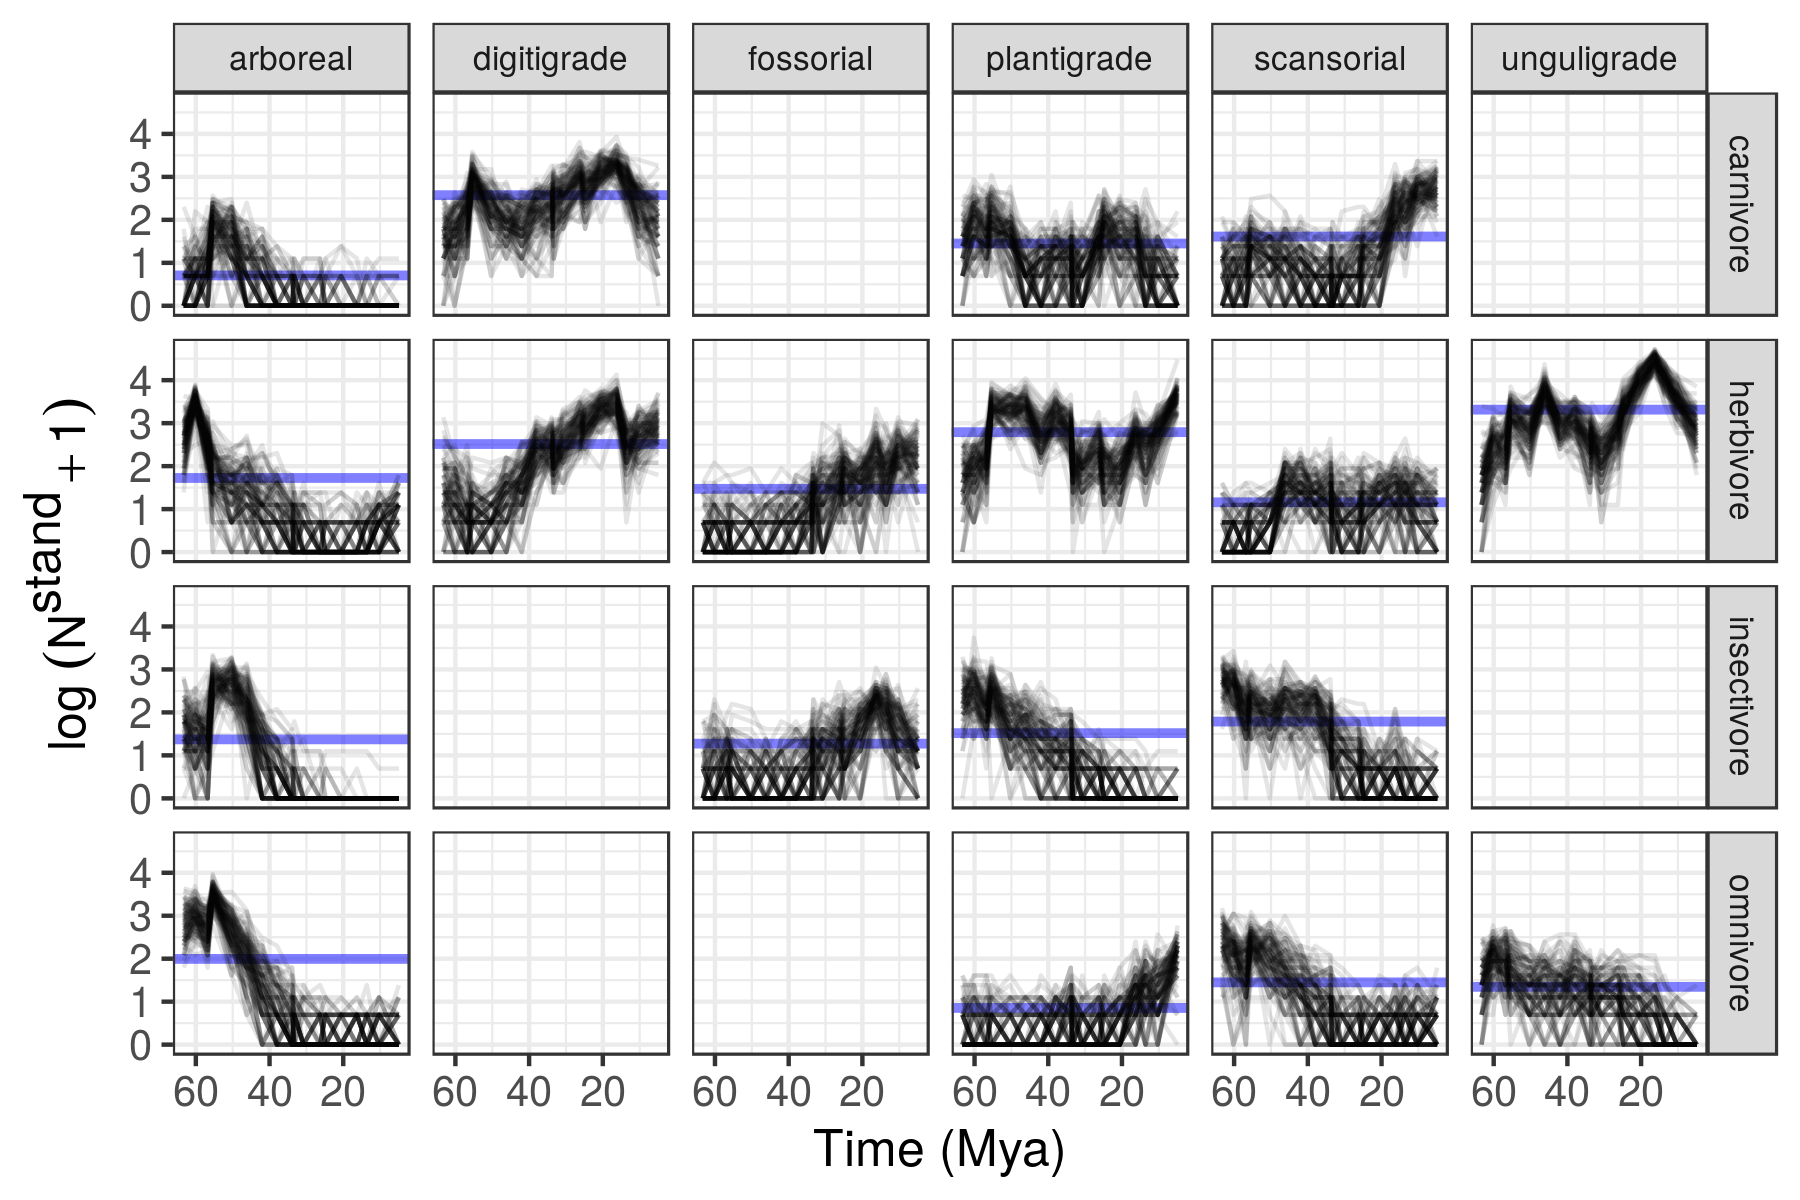
\includegraphics[width=\textwidth,height=0.5\textheight,keepaspectratio=true]{figure/ecotype_diversity}
  \caption[Estimated mammal ecotype log-diversity for the Cenozoic]{Posterior of standing log-diversity of North American mammals by ecotype for the Cenozoic as estimated from the birth-death model; 100 posterior draws are plotted to indicate the uncertainty in these estimates and what is technically plotted is log of diversity plus 1.}
  \label{fig:ecotype_diversity}
\end{figure}



The waxing and waning of the mammal ecotypes is obvious when comparing changes to estimated relative log-mean of diversity (Fig. \ref{fig:ecotype_relative}). While the relative diversity of functional groups changes gradually over time, there are definite patterns associated with a few functional groups and axes of functional diversity that are interesting. There are many expansions and retractions of functional group relative diversity, some of which are coincidental. Only in the case of digitigrade carnivores, plantigrade herbivores, and scansorial omnivores are their functional groups are maintained as relatively constant proportions of the species pool (Fig. \ref{fig:ecotype_relative}).

% increase in the species pool
Eight of the 18 functional groups expand in relative diversity over the Cenozoic (Fig. \ref{fig:ecotype_relative}). Digitigrade herbivores have an obvious increase in relative diversity starting 45Mya, after which it remains a substantial part of the species pool. Fossorial herbivores, and fossorial insectivores increase in relative diversity at approximately 35Mya, after which these groups are maintained as parts of the species pool. Plantigrade omnivores, and scansorial carnivores are both a relatively small fraction of the species pool until approximately 25Mya, after which these functional groups slowly increase in relative diversity for the rest of the time analyzed. Scansorial herbivores expand their relative diversity after approximately 30Mya, after which this functional group has an approximately constant relative diversity. Scansorial insectivores experience in increase in relative diversity after approximately 50Mya. Finally, unlike other functional groups, unguligrade herbivores slowly increase in their relative diversity for the entire Cenozoic.

% decrease in the species pool
Six of the 18 functional groups are estimated to experience a decrease in relative diversity over the Cenozoic (Fig. \ref{fig:ecotype_relative}). As expected from the diversity time-series for the functional groups (Fig. \ref{fig:ecotype_diversity}), the relative diversity of all four arboreal functional groups declines from the beginning of the Cenozoic until approximately 30Mya, after which only arboreal herbivores remain in any capacity (Fig. \ref{fig:ecotype_relative}). In addition to the arboreal groups, there are other functional groups which decrease in relative diversity over the Cenozoic (Fig. \ref{fig:ecotype_relative}). Plantigrade carnivores are a relatively constant portion of the species pool until approximately 10-15Mya, after which this functional group decreases in relative diversity. Plantigrade insectivores decrease in their relative diversity, experience greatest winnowing starting approximately 30-35Mya until 15Mya, after which this functional group becomes absent from the species pool. Finally, unguligrade omnivores begin to decrease in relative diversity starting approximately 20Mya, after which they continue to decrease until they are only a small portion of the relative diversity of the species pool.
\begin{figure}[ht]
  \centering
  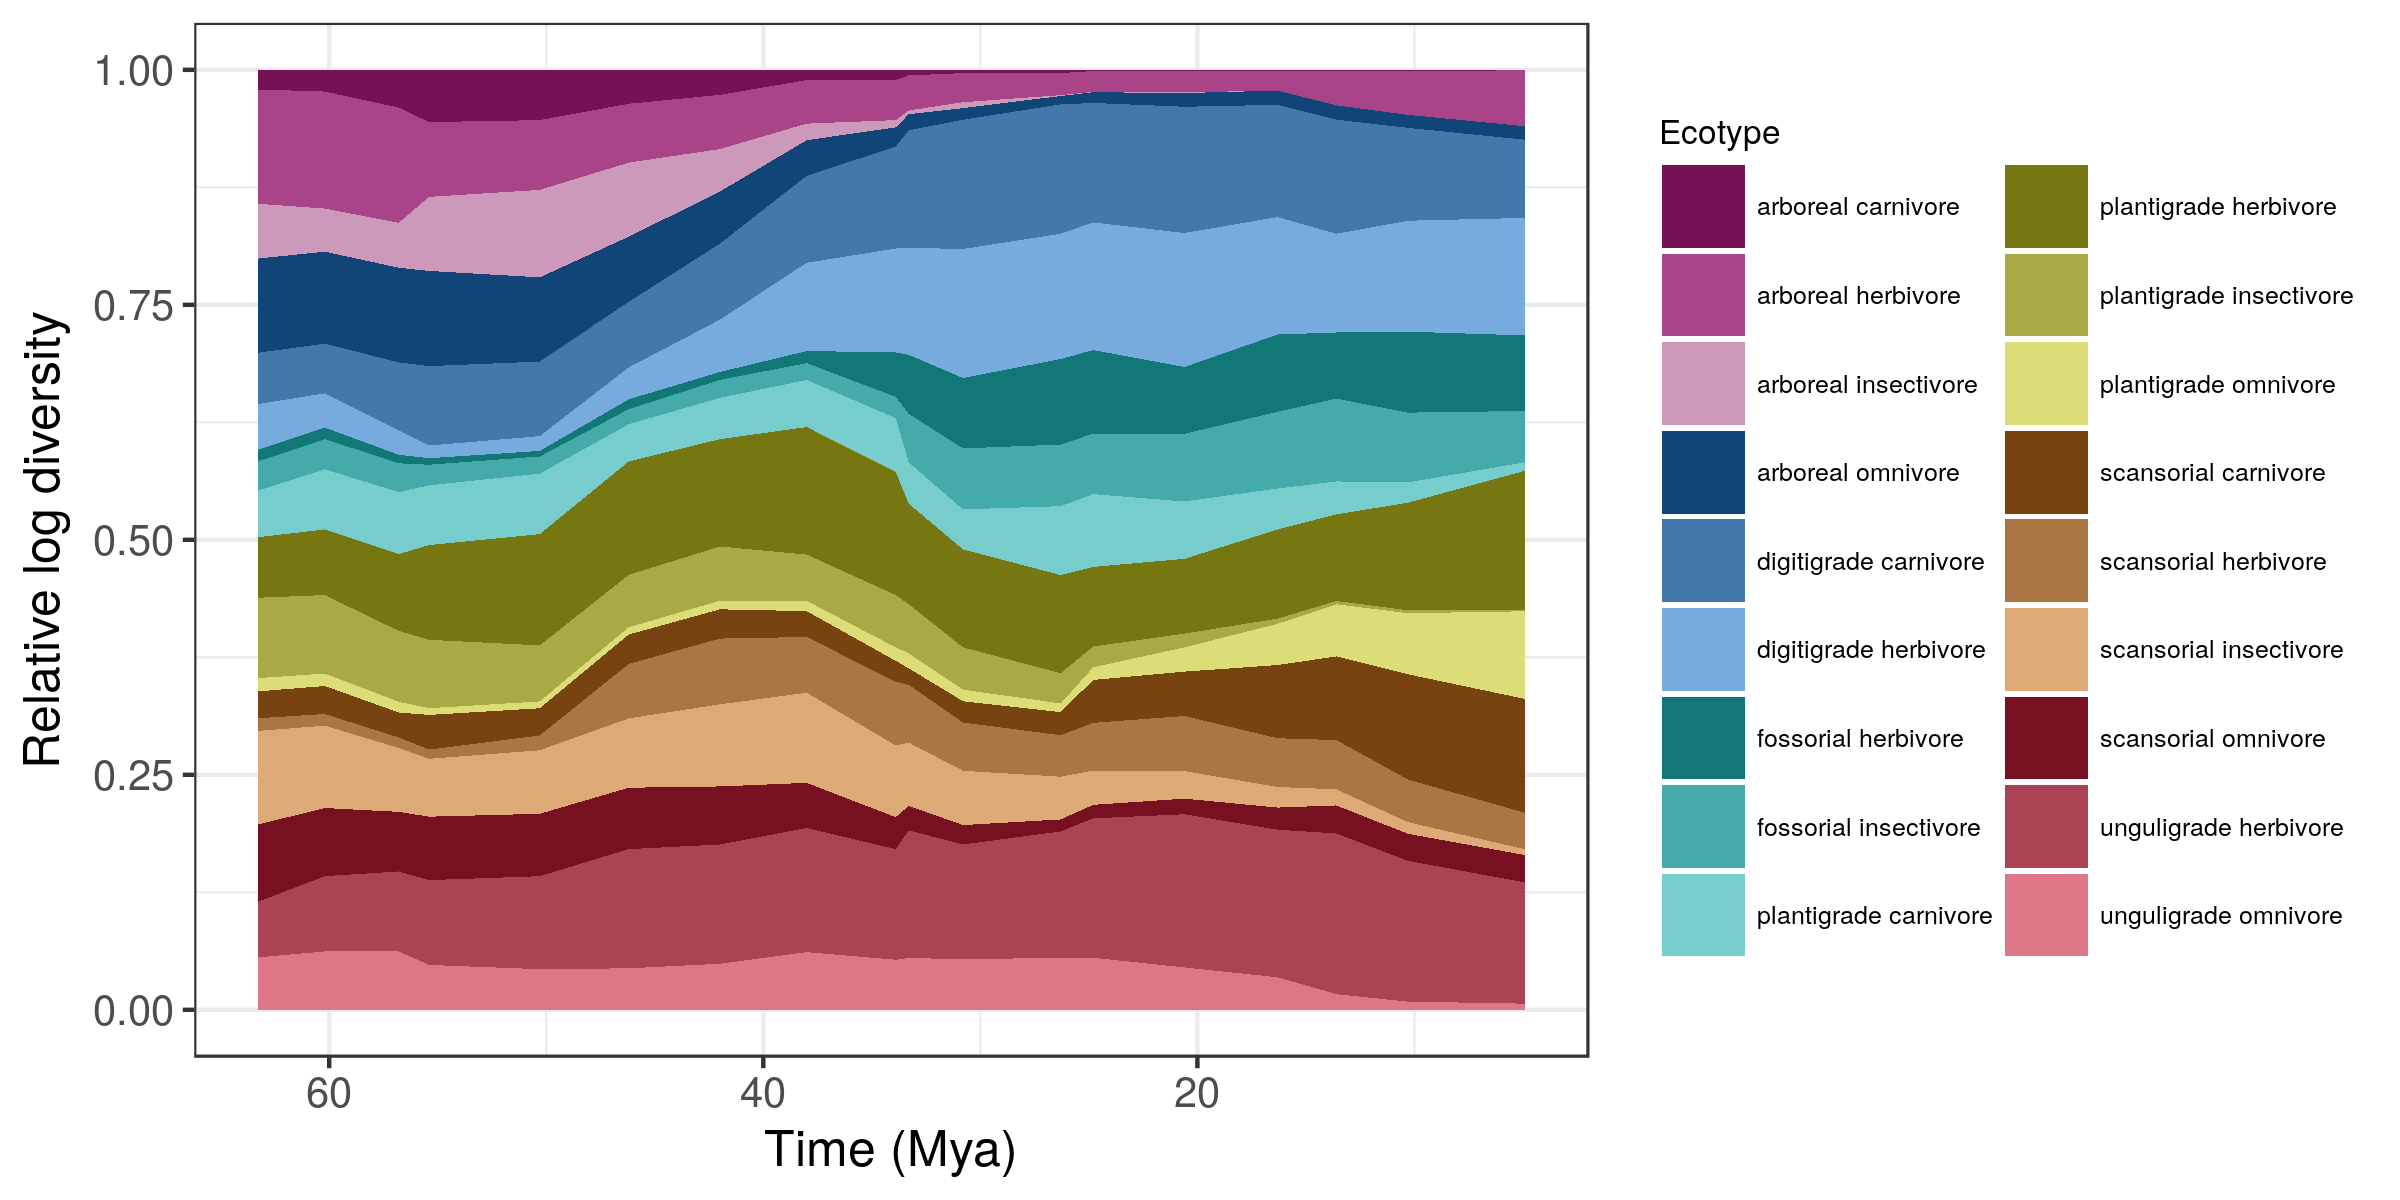
\includegraphics[width=\textwidth,height=0.5\textheight,keepaspectratio=true]{figure/relative_diversity}
  \caption[Relative mammal ecotype log-diversity for the Cenozoic]{Mean posterior estimate of relative log standing diveristy of 18 North American mammal ecotypes for the Cenozoic. These estimates are calculated from 100 posterior estimates of the true occurrence matrix \(z\) as estimated from the birth-death model.}
  \label{fig:ecotype_relative}
\end{figure}


\end{document}

